\documentclass[12pt, openany]{report}
\usepackage[utf8]{inputenc}
\usepackage[T1]{fontenc}
\usepackage{amsmath,amsfonts,amssymb}
\usepackage{amssymb}
\usepackage{multicol}
\usepackage[a4paper,left=2.5cm,right=2.5cm,top=2.5cm,bottom=2.5cm]{geometry}
\usepackage[english]{babel}
\usepackage{libertine}
\usepackage{graphicx}
\usepackage{wrapfig}
\usepackage{tikz}
\usetikzlibrary{shapes.multipart}
\usepackage{algorithm}
\usepackage{algpseudocode}
\usepackage{float}
\usepackage{enumitem}
\usepackage{pythonhighlight}
\usepackage[]{titletoc}
\usepackage{empheq}
\usepackage{titlesec}
\usepackage{mathpazo}
\usepackage{xfrac}
\usepackage{textcomp}
\usepackage{mathtools}
\usepackage{caption}
\usepackage{tabularray}
\usepackage{subcaption}
\usepackage[bottom]{footmisc}
\usepackage{pdfpages}
\usepackage{tabularx}
\usepackage{amsthm}
\usepackage[skins]{tcolorbox}
\titleformat{\chapter}[display]
  {\normalfont\bfseries}{}{0pt}{\Huge}
\usepackage{hyperref}
\newcommand{\hsp}{\hspace{20pt}}
\newcommand{\HRule}{\rule{\linewidth}{0.5mm}}
\newcommand{\R}{\mathbb{R}}
\newcommand{\C}{\mathbb{C}}
\renewcommand{\P}{\mathbb{P}}
\newcommand{\A}{\mathcal{A}}
\newcommand{\Z}{\mathbb{Z}}
\newcommand{\E}{\mathbb{E}}
\theoremstyle{definition}
\newtheorem{thm}{Theorem}[chapter]
\newtheorem{definition}[thm]{Definition}
\newtheorem{lem}[thm]{Lemma}

\hbadness=100000
\begin{document}
\begin{titlepage}
    \begin{sffamily}
    \begin{center}
        
\includegraphics[scale=0.25]{img/page_de_garde.png} \\[1cm]
        \HRule \\[0.4cm]
        { \huge \bfseries LINMA2491 Operational Research \\[0.4cm] }
    
        \HRule \\[1.5cm]
        \textsc{\LARGE Simon Desmidt\\ Issambre L'Hermite Dumont}\\[1cm]
        \vfill
        \vspace{2cm}
        {\large Academic year 2024-2025 - Q2}
        \vspace{0.4cm}
         
        
\includegraphics[width=0.15\textwidth]{img/epl.png}
        
        UCLouvain\\
    
    \end{center}
    \end{sffamily}
\end{titlepage}

\setcounter{tocdepth}{1}
\tableofcontents
\chapter{Definitions and notations}
\begin{itemize}
	\item Given $\Omega$, a sigma-algebra $\A$ is a set of subsets of $\Omega$, with the elements called events, such that:
	\begin{itemize}
		\item $\Omega \in \A$
		\item if $A \in \A$ then also $\Omega - A \in \A$
		\item if $A_i \in \A$ for $i = 1,2, \dots$ then also $\cup_{i=1}^\infty A_i \in \A$
		\item if $A_i \in \A$ for $i = 1,2, \dots$ then also $\cap_{i=1}^\infty A_i \in \A$
	\end{itemize}
	\item Consider: 
	\begin{figure}[H]
		\centering
		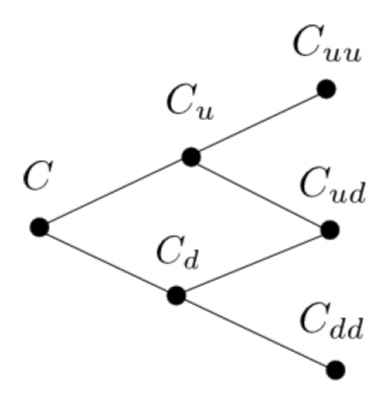
\includegraphics[scale=0.25]{img/space.jpg} 
	\end{figure}
	\begin{itemize}
		\item The state space is the set of all values of the system at each stage. 
		\begin{equation}
			S_0 = \{C\},\qquad S_1 = \{C_u, C_d\},\qquad S_2 = \{C_{uu}, C_{ud}, C_{dd}\}
		\end{equation}
		\item  The sample space is the set of all possible combination of the system.
		\begin{equation}
			\Omega = S_0 \times S_1 \times S_2 = \{(C, C_u, C_{uu}), (C, C_u, C_{ud}), (C, C_u, C_{dd}), \dots\}
		\end{equation}
	\end{itemize}
	\item The power set of $\Omega$ is the set of all of the subsets, denoted $\mathcal{B}(\Omega)$.
	\item The probability space is the triplet $(\Omega, \A, P)$ where $P$ is a probability measure.
	\begin{itemize}
		\item $P(\emptyset) = 0$
		\item $P(\Omega) = 1$
		\item $P(\cup_{i=1}^\infty A_i) = \sum_i P(A_i)$ if $A_i$ are disjoint
	\end{itemize} 
	\item $\forall t, A_t$ is the set of events on which we have information at stage $t$. For example, $A_0 = \{C\}$, $A_1 = \{C, C_u, C_d\}$. Thus is it evident that $ t_1 \leq t_2 \Rightarrow \A_{t_1} \subseteq \A_{t_2}$
	\item Consider the following problem with $x \in \R^n$ and domain $\mathcal{D}$:
	\begin{equation}
		\begin{aligned}
			&\min f_0(x), \qquad s.t.\\
			&f_i(x) \leq 0, i = 1, \dots, m\\
			&h_j(x) = 0, j = 1, \dots, p
		\end{aligned}
	\end{equation}
	Then the Lagrangian function is defined as $L: \R^n \times \R^m \times \R^p \to \R$:
	\begin{equation}
		L(x, \lambda, \nu) = f_0(x) + \sum_{i=1}^m \lambda_i f_i(x) + \sum_{j=1}^p \nu_j h_j(x)
	\end{equation}
	\item  The Lagrange dual function is defined as $g: \R^m \times \R^p \to \R$:
	\begin{equation}
		g(\lambda, \nu) = \inf_{x \in \mathcal{D}} L(x, \lambda, \nu)
	\end{equation}
	\item The Lagrange dual problem is a lower bound on the optimal value of the primal problem
	\item Lagrange relaxation of Stochastic Programs, consider the two problems:
	\begin{equation}
		\begin{aligned}
			\min f_1(x) + \E_\omega[f_2(y(\omega), \omega)] \qquad & \qquad \min f_1(x) + \E_\omega[f_2(y(\omega), \omega)]\\
			s.t \qquad h_{1i}(x) \leq 0, i = 1, \dots, m_1 \qquad & \qquad s.t. \qquad h_{1i}(x) \leq 0, i = 1, \dots, m_1\\
			h_{2i}(x,y(\omega),\omega) \leq 0, i = 1, \dots, m_2 \qquad & \qquad h_{2i}(x(\omega),y(\omega),\omega) \leq 0, i = 1, \dots, m_2\\
			& \textcolor{red}{\qquad x(\omega) = x} 
		\end{aligned}
	\end{equation}
	The red constraint is the non-anticipativity constraint, it transforms the deterministic variable into a stochastic variable. \textcolor{red}{A VERIFIER}
	\item The dual of a stochastic program is:
	\begin{equation}
		\begin{aligned}
			& g(\nu) = g_1(\nu) + \E_\omega(g_2(\nu, \omega))\\
			where \qquad &  \\
			& g_1(\nu) = \inf f_1(x) + \left( \displaystyle \sum_{\omega \in \Omega} \nu(\omega) \right)^T x\\
			& s.t. \quad h_{1i} (x) \leq 0, i = 1, \dots, m_1\\
			and \qquad &  \\
			& g_2(\nu, \omega) = \inf f_2(y(\omega) \omega) - \nu x(\omega)\\
			& s.t. \quad h_{2i}(x(\omega), y(\omega), \omega) \leq 0, i = 1, \dots, m_2
		\end{aligned}
	\end{equation}
	\item  With $p^*$ the solution of the primal problem and $d^*$ the solution of the dual problem, we have:
	\begin{itemize}
		\item Weak duality: $d^* \leq p^*$
		\item Strong duality: $d^* = p^*$
	\end{itemize}
	\item The KKT conditions are necessary and sufficient for optimality in convex optimization, there aren't unique. They are:
	\begin{itemize}
		\item Primal constraint: $f_i(x) \leq 0, i = 1, \dots, m$, $h_j(x) = 0, j = 1, \dots, p$
		\item Dual constraint: $\lambda \geq 0$
		\item Complementarity slackness: $\lambda_i f_i(x) = 0, i = 1, \dots, m$
		\item Gradient of the Lagrangian: $\nabla_x L(x, \lambda, \nu) = 0$
	\end{itemize}
	\item An extreme point of a polyhedron $P$ is a point $x\in P$ such that it cannot be expressed as a linear combination of two distinct points in $P$, i.e. an extreme point is a vertex of the polyhedron.
	\item An extreme ray of a polyhedron $P$ is $\sigma\in \R^n$ such that for all $x\in P$, for all $\lambda \in [0,1]$, 
	\begin{equation}\label{eq:extreme}
		(x+\lambda \sigma)\in P
	\end{equation}
	i.e. it is a direction in which we can travel infinitely without leaving the polyhedron. 
\end{itemize}
\section{Reminders on subgradients}
$\pi$ is a subgradient of the function $g$ at $u$ if 
\begin{equation}
	g(w)\ge g(u)+ \pi^T(w-u)\qquad \forall w
\end{equation}
If $g=\max \{g_1,g_2\}$ with $g_{1,2}$ convex and differentiable, the subgradient of $g$ at $u_0$ is 
\begin{itemize}
	\item $\pi=\nabla g_1(u_0)$ if $g_1(u_0)>g_2(u_0)$
	\item $\pi=\nabla g_2(u_0)$ if $g_2(u_0)>g_1(u_0)$
	\item The line segment $[\nabla g_1(u_0),\nabla g_2(u_0)]$ if $g_1(u_0)=g_2(u_0)$
\end{itemize}
The subdifferential of $g$ at $u$ is the set of all subgradients of $g$ at $u$, denoted $\partial g(u)$. If $g$ is convex, then its subdifferential is nonempty on its domain, and $g$ is differentiable at $u$ if its $\partial g(u) = \{\pi\}$. 
\subsection{Use in duality}
Define $c(u)$ as the optimal value of 
\begin{equation}
	\begin{aligned}
		c(u)&=\min f_0(x)\\
		f_i(x) &\le u_i \qquad i=1,\dots,m\\
	\end{aligned}
\end{equation}
where $x\in dom f_0$ and $f_0,f_i$ are convex functions.
\begin{itemize}
	\item $c(u)$ is convex;
	\item If strong duality holds, denote $\lambda^\star$ as the maximizer of the dual function 
	\begin{equation}
		\inf_{x\in dom f_0} (f_0(x) - \lambda^T(f(x)-u))
	\end{equation}
	for $\lambda \le 0$. Then, $\lambda^\star \in \partial c(u)$. $\lambda_i$ represents the sensitivity of $c(u)$ to a marginal change in the right-hand side of the $i$-th constraint. 
\end{itemize}
\chapter{Modelling}
\section{Introduction}
\begin{itemize}
	\item  For a certain sequence of events $x \to \omega \to y(\omega)$, where $\omega$ is the uncertainty,
	\begin{itemize}
		\item A first-stage decision is a decision that is made before the uncertainty is revealed (i.e. in $x$);
		\item A second-stage decision is a decision that is made after the uncertainty is revealed (i.e. in $y(\omega)$).
	\end{itemize}
	\item We can have the following mathematical formulation:
	\begin{equation}\label{eq:TSSLP_formulation}
		\begin{aligned}
			\min c^T x &+ \E[q(\omega)^T y(\omega)]\\
			Ax &= b\\
			T(\omega) x &+ W(\omega)y(\omega) = h(\omega)\\
			x \geq 0&, y(\omega) \geq 0
		\end{aligned}
	\end{equation}
	\begin{itemize}
		\item First-stage decision variable: $x \in \R^{n_1}$
		\item First-stage parameter: $c \in \R^{n_1}$, $b \in \R^{m_1}$ and $A \in \R^{m_1 \times n_1}$
		\item Second-stage decision: $y(\omega) \in \R^{n_2}$
		\item Second-stage data: $q(\omega) \in \R^{n_2}$, $h(\omega) \in \R^{m_2}$ and $T(\omega) \in \R^{m_2 \times n_1}$, $W(\omega) \in \R^{m_2 \times n_2}$
	\end{itemize}
\end{itemize}
\section{Representations}
\subsection{Scenario Trees}
A scenario tree is a graphical representation of a Markov process $\{\xi_t\}_{t\in \Z}$, where the nodes are the history of realizations ($\xi_{[t]}=(\xi_1,\dots,\xi_t)$), and the edges are the transitions from $\xi_{[t]}$ to $\xi_{[t+1]}$.
\begin{itemize}
	\item We denote the root as $t=1$;
	\item An ancestor of a node $\xi_{[t]}$, $A(\xi_{[t]})$ is a unique adjacent node which precedes $\xi_t$;
	\item The children of a node, $C(\xi_{[t]})$ are the nodes that are adjacent to $\xi_{[t]}$ and occur at stage $t+1$.
\end{itemize}
\begin{figure}[H]
	\centering 
	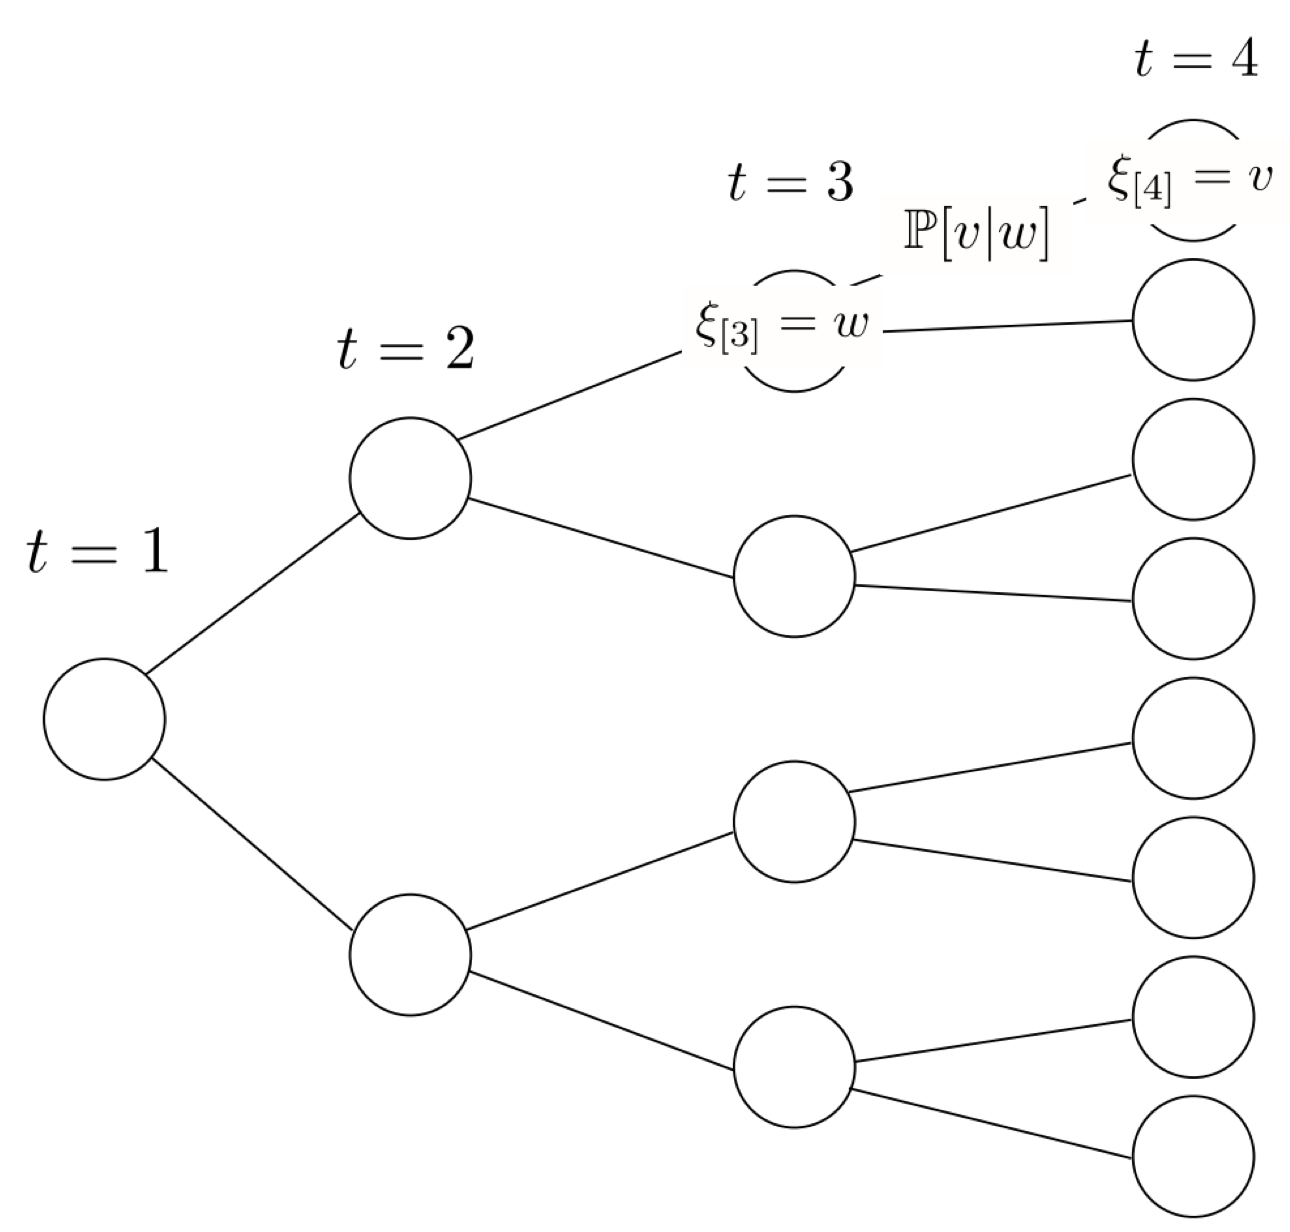
\includegraphics[width = .3\textwidth]{img/tree.png}
\end{figure}
\subsection{Lattice}
A lattice is a graphical representation of a Markov process $\{\xi_t\}_{t\in \Z}$, where the nodes are the realizations $\xi_t$ and the edges correspond to the transitions from $\xi_t$ to $\xi_{t+1}$. 
\begin{figure}[H]
	\centering 
	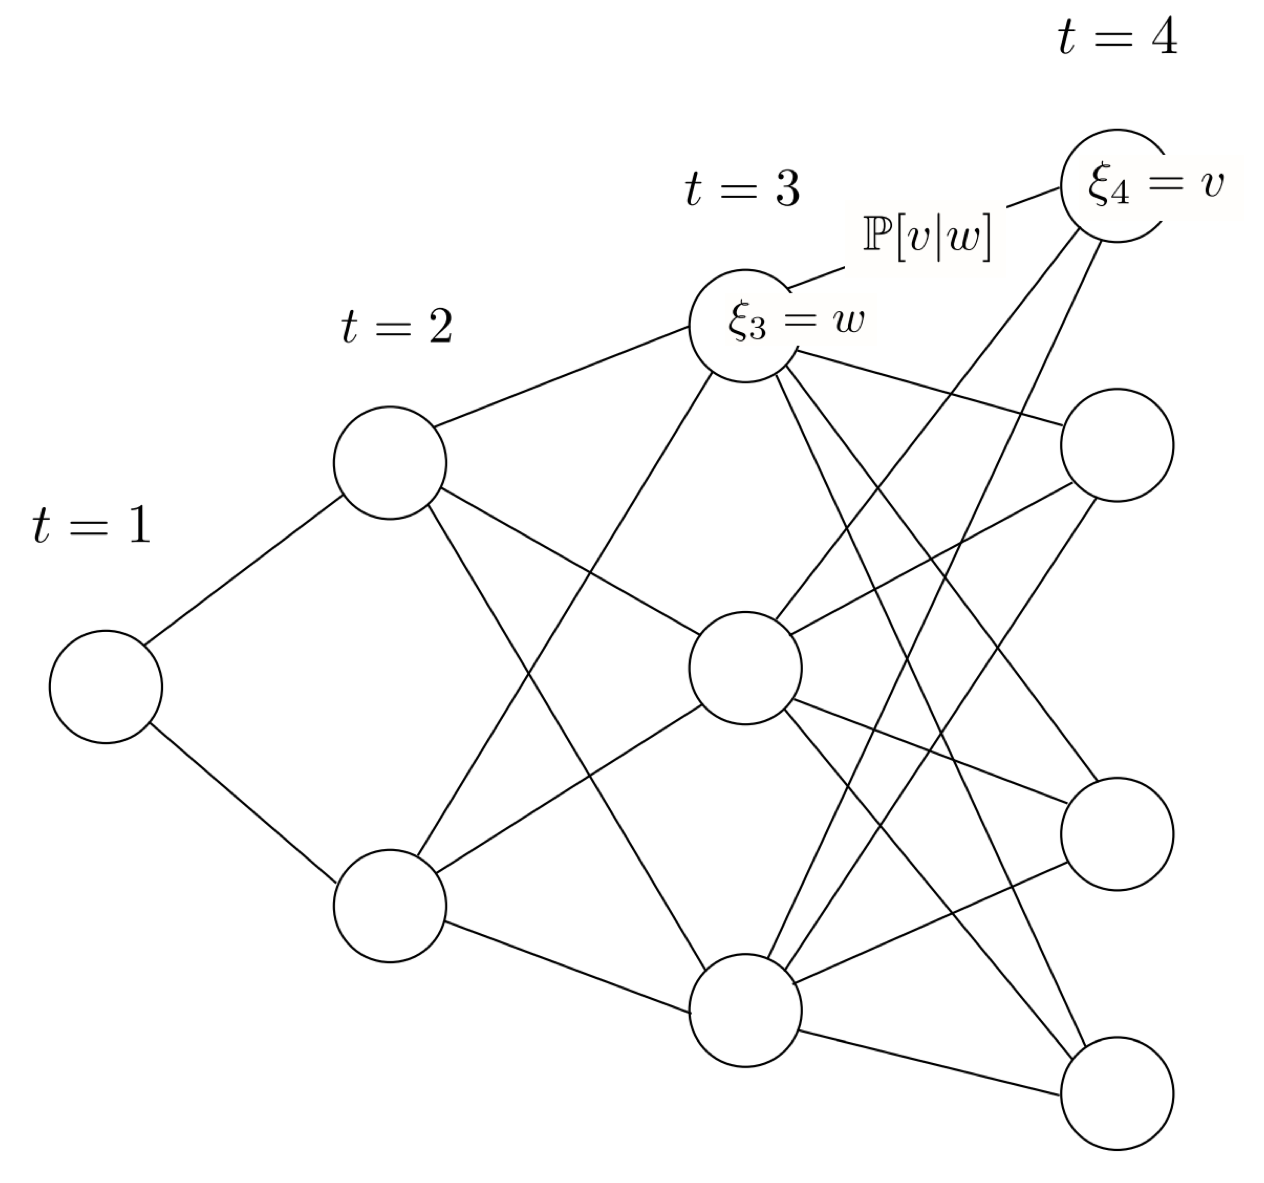
\includegraphics[width = .3\textwidth]{img/lattice.png}
\end{figure}
\subsection{Serial Independence}\label{sec:serial_ind}
A process satisfies serial independence if, for every stage $t$, $\xi_t$ has a probability distribution that does not depend on the history of the process. Thus, the probability measure is 
\begin{equation}
	\P\left[\xi_t(\omega)=i\left|\xi_{[t-1]}(\omega)\right.\right] = p_t(i) \qquad \forall \ \xi_{[t-1]}\in\Xi_{[t-1]}, i\in\Xi_t
\end{equation}
\section{Multi Stage Stochastic Linear Program}\label{sec:st}
\subsection{Notation}
\begin{itemize}
	\item Probability space: $(\Omega, 2^\Omega, \P)$ with filtration $\{\A\}_{t\in \{1, \dots, H\}}$
	\item $c_t(\omega) \in \R^{n_t}$: cost coefficients
	\item $h_t(\omega) \in \R^{m_t}$: right-hand side parameters
	\item $W_t(\omega) \in \R^{m_t \times n_t}$: coefficients of $x_t(\omega)$
	\item $T_{t-1}(\omega) \in \R^{m_t \times n_{t-1}}$: coefficients of $x_{t-1}(\omega)$
	\item $x_t(\omega)$: set of state and action variables in period $t$
	\item We implicitly enforce non-anticipativity by requiring that $x_t$ and $\xi_t$ are adapted to filtration $\{\mathcal{A}\}_{t\in \{1, \dots, H\}}$ 
	\item $\forall A \in \mathcal{A}_k \setminus \mathcal{A}_{k-1}, \: x_t(\omega_1)=x_t(\omega_2) \: \forall\omega_1,\omega_2 \in A$
	\item [$\to$] Note: The filtration $\mathcal{A}_t$ represents what is distinguishable at the time of observation; it reveals the incertainty at each time $t$. 
\end{itemize}
\begin{equation}
	\mathcal{A}_t = \mathcal{A}_{t-1}\cup \left\{\cup_{E_i\in \Omega}\left\{E_i, \Omega\setminus \{E_i\}\right\}\right\} \qquad E_i = \{S_1,\dots,S_{i-1},s_i,S_{i+1},\dots, S_H\}
\end{equation}
where $s_i$ is a realisation of the state set $S_i$.
\subsection{General formulation of the MSLP}
The extended formulation of the MSLP is: 
\begin{equation}
	\begin{aligned}
		&\min c_1^Tx_1 + \E[c_2(\omega)^T x_2(\omega)+ \dots + c_H(\omega)^Tx_H(\omega)]\\
		&s.t. \quad W_1x_1 = h_1\\
		&T_1(\omega)x_1 + W_2(\omega)x_2(\omega) = h_2(\omega), \omega \in \Omega\\
		&\qquad \qquad \vdots\\
		&T_{t-1}(\omega)x_{t-1}(\omega) + W_t(\omega)x_t(\omega) = h_t(\omega), \omega \in \Omega\\
		&\qquad \qquad \vdots\\
		&T_{H-1}(\omega)x_{H-1}(\omega) + W_H(\omega)x_H(\omega) = h_H(\omega), \omega \in \Omega\\
		&x_1 \geq 0, x_t(\omega) \geq 0, t=2, \dots, H
	\end{aligned}
\end{equation}
We can now consider two specific instantiations of the MSLP: the scenario tree (MSLP-ST) and the lattice (MSLP-L). Using these notations:
\begin{itemize}
	\item $\omega_t \in S_t$ : index in the support $\Xi_t$ of random input $\xi_t$
	\item $\omega_{[t]} \in S_1 \times \dots \times S_t$ (interpretation: index in $\Xi_{[t]} = \Xi_1 \times \dots \times \Xi_t$, which is the history of realizations, up to period $t$)
\end{itemize}
\subsection{Scenario Tree formulation}
\begin{equation}\label{eq:scenario_tree}
	 \begin{aligned}
		&\min c_1^Tx_1 + \E\left[c_2(\omega_{[2]})^T x_2(\omega_{[2]})+ \dots + c_H(\omega_{[H]})^Tx_H(\omega_{[H]})\right]\\
		&s.t. \quad W_1x_1 = h_1\\
		&T_1(\omega_{[2]})x_1 + W_2(\omega_{[2]})x_2(\omega_{[2]}) = h_2(\omega_{[2]}), \omega_{[2]} \in S_1 \times S_2\\
		&\qquad \qquad \vdots\\
		&T_{t-1}(\omega_{[t]})x_{t-1}(\omega_{[t-1]}) + W_t(\omega_{[t]})x_t(\omega_{[t]}) = h_t(\omega_{[t]}), \omega_{[t]} \in S_1 \times \dots \times S_t\\
		&\qquad \qquad \vdots\\
		&T_{H-1}(\omega_{[H]})x_{H-1}(\omega_{[H-1]}) + W_H(\omega_{[H]})x_H(\omega_{[H]}) = h_H(\omega_{[H]}), \omega_{[H]} \in S_1 \times \dots \times S_H\\
		&x_1 \geq 0, x_t(\omega_{[t]}) \geq 0, t=2, \dots, H
	 \end{aligned}
\end{equation}
\subsection{Lattice formulation}
\begin{equation}
	\begin{aligned}
		&\min c_1^Tx_1 + \E\left[c_2(\omega_{2})^T x_2(\omega_{[2]})+ \dots + c_H(\omega_{H})^Tx_H(\omega_{[H]})\right]\\
		&s.t. \quad W_1x_1 = h_1\\
		&T_1(\omega_{2})x_1 + W_2(\omega_{2})x_2(\omega_{[2]}) = h_2(\omega_{2}), \omega_{[2]} \in S_1 \times S_2\\
		&\qquad \qquad \vdots\\
		&T_{t-1}(\omega_{t})x_{t-1}(\omega_{[t-1]}) + W_t(\omega_{t})x_t(\omega_{[t]}) = h_t(\omega_{t}), \omega_{[t]} \in S_1 \times \dots \times S_t\\
		&\qquad \qquad \vdots\\ 
		&T_{H-1}(\omega_{H})x_{H-1}(\omega_{[H-1]}) + W_H(\omega_{H})x_H(\omega_{[H]}) = h_H(\omega_{H}), \omega_{[H]} \in S_1 \times \dots \times S_H\\
		&x_1 \geq 0, x_t(\omega_{[t]}) \geq 0, t=2, \dots, H
	\end{aligned}
\end{equation}
\begin{itemize}
	\item [$\rightarrow$] Note: There exists some relations to other decision making problems such as statistical decision theory, dynamic programming, online optimization and stochastic control.
\end{itemize}

\chapter{Performance}
\section{Notations}
Using \eqref{eq:TSSLP_formulation}, let's define the following:
\begin{itemize}
	\item $z(x,\xi) = c^Tx+Q(x,\xi)+\delta(x|K_1)$
	\item $Q(x,\xi) = \displaystyle \min_y\{q(\omega)^Ty\ |\ W(\omega)y=h(\omega)-T(\omega)x\}$
	\item $K_1 = \{x|Ax=b,x\geq0\}$ is the set of feasible first-stage decisions
	\item $K_2(\omega)=\{x\ |\ \exists y\geq0:W(\omega)y=h(\omega)-T(\omega)x\}$ is the set of first-stage decisions that have a feasible reaction in the second stage for $\omega \in \Omega$
	\item It is possible that $z(x,\xi) = + \infty$ (if $x \notin K_1 \cap K_2(\omega)$)
	\item It is possible that $z(x,\xi) = - \infty$ (unbounded below)
\end{itemize}
\section{Expected value of perfect information}
There are 2 tactics:
\begin{itemize}
	\item \textbf{wait-and-see} value is the expected value of reacting with perfect foresight (we know everything that will happen) $x^*(\xi)$ to $\xi$: 
	\begin{equation}
		WS = \E[\displaystyle \min_x z(x,\xi)] = \E[z(x^*(\xi),\xi)]
	\end{equation}
	\item \textbf{here-and-now} value is the expected value of the recourse problem (remove non-anticipativity constraint):
	\begin{equation}
		SP = \displaystyle \min_x \E[z(x,\xi)]
	\end{equation}
\end{itemize}
The \textbf{expected value of perfect information} is like the value we give to getting a perfect forecast for the future and is thus defined like this:
\begin{equation}
	EVPI = SP - WS
\end{equation}
\begin{itemize}
	\item [$\to$] Note: for a maximum, the difference is reversed, and the inequalities that are coming are too.
\end{itemize}
\section{The value of the stochastic solution}
Here too there are 2 tactics:
\begin{itemize}
	\item \textbf{expected value problem}
	\begin{equation}
		EV = \displaystyle \min_x z(x,\bar{\xi}) \qquad \bar \xi = \E[\xi]
	\end{equation}
	and its \textbf{expected value solution} is noted $x^*(\bar{\xi})$.
	\item \textbf{expected value of using the EV solution} measures the performance of $x^*(\bar{\xi})$:
	\begin{equation}
		EEV = \E[z(x^*(\bar{\xi}),\xi)]
	\end{equation}
\end{itemize}
% We also have $EEV \geq SP$.\\
The \textbf{value of the stochastic solution} is noted like this:
\begin{equation}
	VSS = EEV - SP
\end{equation}
\section{Basic inequalities}
\subsection{Crystal Ball}
For every $\xi$, we have $z(x^*(\xi),\xi) \leq z(x^*,\xi)$ where $x^*$ is the optimal solution to the stochastic program. And if we take the expectation of this inequality, we have $WS \leq SP$, because $WS$ is a relaxation. It explains that we can do better with a crystal ball. 
\subsection{Lazy solution}
Knowing that $x^*$ is the optimal solution of $\displaystyle \min_x \E[z(x,\xi)]$ and $x^*(\bar{\xi})$ is a solution but not necessarily optimal then we have $SP \leq EEV$, because:
\begin{equation}
	\displaystyle \min_x \E[z(x,\xi)] = SP \leq EEV = \E[z(x^*(\bar{\xi}),\xi)]
\end{equation}
\subsection{Link between all the values}
We know that:\\
\begin{minipage}{.5\textwidth}
	\begin{itemize}
		\item $VSS \geq 0$
		\item $EVPI \geq 0$
		\item $VSS \leq EEV - EV$
	\end{itemize}
\end{minipage}
\begin{minipage}{.5\textwidth}
	\begin{itemize}
		\item $EVPI \leq EEV -EV$
		\item If $EEV - EV = 0$ then $VSS = EVPI = 0$
	\end{itemize}
\end{minipage}
and the inequalities can be summarized in the following diagram:
\begin{figure}[H]
	\centering
	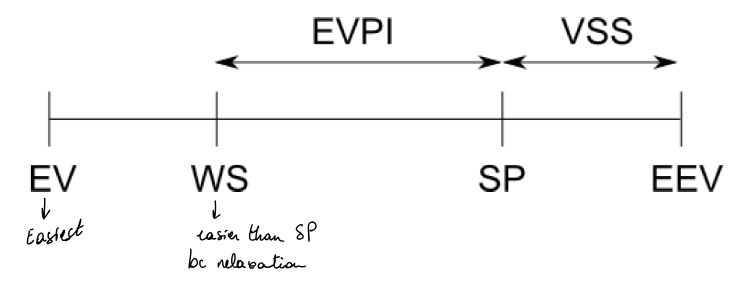
\includegraphics[scale=0.5]{img/link_ineq.png}
\end{figure}
\section{Bounds on EVPI and VSS}
First let's introduce the pairs subproblem of $\xi^r$ and $\xi^k$:
\begin{equation}
	\begin{aligned}
		\min \: &z^P (x, \xi^r,\xi^k) = c^Tx + p^rq^Ty(\xi^r) + (1-p^r)q^Ty(\xi^k)\\
		s.t. \: &Ax = b\\
		&Wy(\xi^r) = \xi^r-Tx\\
		&Wy(\xi^k) = \xi^k-Tx\\
		&x,y\geq0
	\end{aligned}
\end{equation}
\begin{itemize}
	\item $(\bar{x}^k , \bar{y}^k , y(\xi^r ))$ denotes an optimal solution to the problem and $z^k$ is the optimal objective function value $z^P (\bar{x}^k , \bar{y}^k , y(\xi^k ))$
	\item $z^P (x, \xi^r , \xi^r)$ corresponds to the deterministic optimization against the
	reference scenario
	\item if $\xi^r \notin \Xi$, $p^r = 0$ and $z^P (x, \xi^r , \xi^k ) = z(x, \xi^k )$
\end{itemize}
The \textbf{sum of pairs expected value (SPEV)}:
\begin{equation}
	SPEV = \frac{1}{1-p^r} \sum_{k=1,k \neq r}^{K} p^k \min z^P(x, \xi^r,\xi^k)
\end{equation}
When $\xi^r \notin \Xi$ then $SPEV = WS$: When $p^r = 0, z^P(x,\xi^r,\xi^k)$ coincides with $z(x,\xi^k)$. Therefore $SPEV = \sum_{k=1}^{K} p^k \min_x z(x,\xi^k) = WS$.\\
We then know $WS \leq SPEV \leq SP$.
\subsection{Upper bound on SP: EVRS and EPEV}
\begin{itemize}
	\item The \textbf{expected value of the reference scenario} is $EVRS =  \E_\xi(z(\bar{x}^r,\xi))$, where $\bar{x}^r$ is the optimal solution to $z(x,\xi^r)$.
	\item The \textbf{expectation of pairs of expected value} is defined as \[EPEV = \min_{k=1,\dots,K\cup\{r\}}\E_\xi(z(\bar{x}^k,\xi))\] where $(\bar{x}^k,\bar{y}^k, y(\xi^K))$ is the optimal solution to the pairs subproblem of $\xi^r$ and $\xi^k$.
\end{itemize}
As $SP,EPEV,EVRS$ are the optimal values of $\min_x \E_\xi z(x,\xi)$ over smaller feasible sets:
\begin{equation}
	SP \leq EPEV \leq EVRS
\end{equation}
Because
\begin{itemize}
	\item $SP$: $x \in K_1 \cap K_2$
	\item $EPEV$: $x \in K_1 \cap K_2 \cap \{\bar{x}^k,k=1,\dots,K\cup\{r\}\}$
	\item $EVRS$: $x \in \bar{x}^r \cap K_1 \cap K_2$
\end{itemize}
\section{Estimations of WS and EEV}
An estimation of WS and EEV can be done through a sample mean approximation: from samples $\xi_i = \xi(\omega_i)$ for $i=1,\dots,K$, 
\begin{enumerate}
	\item Compute $x^\star (\bar \xi)$;
	\item Compute $WS_i = z(x^\star (\xi_i), \xi_i)$ and $EEV_i = c^Tx^\star (\xi_i) + Q(x^\star (\bar \xi), \xi_i)$;
	\item Estimate $\Bar{WS} = \frac{1}{K}\sum_{i=1}^K WS_i$ and $\bar{EEV} = \frac{1}{K}\sum_{i=1}^K EEV_i$.  
\end{enumerate}
\subsection{Central Limit Theorem}
Suppose $\{X_1, \dots, X_K\}$ is a sequence of iid rv with $\E[X_i]=\mu$ and $Var[X_i] = \sigma^2<\infty$. Then, as $n$ approaches infinity, $\sqrt{n}(S_n-\mu)$ converge in distribution to a normal $\mathcal{N}(0,\sigma^2)$:
\begin{equation}
	\sqrt{n}\left(\left(\frac{1}{n}\sum_{i=1}^n X_i\right)-\mu\right) \xrightarrow{d} \mathcal{N}(0,\sigma^2)
\end{equation}
The central limit theorem is useful to decrease the importance of rare but extreme events. 
\subsection{Importance sampling}
Suppose we wish to estimate $\E[C(\omega)]$, where $\omega$ is distributed according to $f(\omega)$ and estimates $\E[C(\omega)]$ with $\displaystyle \sum_{i=1}^N \frac{1}{N}C(\omega_i)$. A sample average pulls samples $\omega_i$ according to the distribution function $f(\omega)$, while the importance sampling pulls the samples $\omega_i$ according to the distribution $\displaystyle g(\omega) = \frac{f(\omega)C(\omega)}{\E[C(\omega)]}$, where the $\E[C(\omega)]$ is an approximation of the real expectation. It then estimates $\E[C(\omega)]$ with $\displaystyle \sum_{i=1}^N \frac{1}{N}\frac{f(\omega_i)C(\omega_i)}{g(\omega_i)}$. 
\chapter{Benders Decomposition}
\section{Cutting plane methods}
A cutting plane method is an optimisation method based on the idea of iteratively refining the objective function, or a set of feasible constraints of a problem through linear inequalities (see LINMA2450). 
\subsection{Nomenclature}
\begin{itemize}
	\item The benders decomposition is a specific method for obtaining the cutting planes when $F(x)$ is the value function of a second-stage linear program. 
	\item The L-shaped method is a specific instance of Benders decomposition when the second-stage linear program is decomposable into a set of scenarios.
	\item The multi-cut L-shaped method is an alternative to the L-shaped method which generates multiple cutting planes at step 1 of Kelley's method (see \ref{sec:Kelley}). 
\end{itemize}
\subsection{Kelley's Cutting Plane Algorithm}\label{sec:Kelley}
This algorithm is designed to solve convex but non-differentiable optimization problems of the form
\begin{equation}
	\begin{aligned}
		z^\star &= \min c^Tx + F(x)\\
		\text{s.t. }& x\in X\\
	\end{aligned}
\end{equation}
where $X\subseteq \R^n$ is convex and compact, $F:\R^n\to \R$ is convex and $c\in \R^n$ is a parameter vector. \\
Let us define the following for algorithm \ref{algo:Kelley}
\begin{itemize}
	\item $L_k:\R^n\to \R$ a lower bound function of $F(x)$ at iteration $k$;
	\item $L_k$ a lower bound of $z^\star$ at iteration $k$;
	\item $U_k$ an upper bound $U_k$ of $z^\star$ at iteration $k$.
\end{itemize}
\begin{algorithm}
    \caption{Kelley's Cutting plane algorithm}
	\label{algo:Kelley}
    \begin{algorithmic}[1]
    \State \textbf{Step 0:} Set $k=0$ and assume $x_1\in X$ is given. Set $L_0(x)=-\infty$ for all $x\in X$, $U_0 = c^Tx_1 + F(x_1)$, and $L_0 = -\infty$.
	\State \textbf{Step 1:} Set $k=k+1$. Find $a_k\in \R$ and $b_k\in \R^n$ such that \[F(x_k)=a_k+b_k^Tx_k\] \[F(x)\ge a_k + b_k^Tx\qquad x\in X\]
	\State \textbf{Step 2:} Set \[U_k = \min(U_{k-1},c^Tx_k + F(x_k))\] and \[L_k(x) = \max(L_{k-1}(x),a_k+b_k^Tx) \qquad x\in X\]
	\State \textbf{Step 3:} Compute \[L_k = \min_{x\in X} L_k(x) + c^Tx\] and denote $x_{k+1}$ as the optimal solution of this problem.
	\State \textbf{Step 4:} If $U_k - L_k =0$, stop. Otherwise, go to step 1.
    \end{algorithmic}
\end{algorithm}
\section{Context and description}
Consider the following optimization problem:
\begin{equation}
	\begin{aligned}
		z^\star &= \min c^Tx + q^Ty\\
		Ax&=b\\
		Tx + Wy&=h\\
		x, y\geq0\\
	\end{aligned}
\end{equation}
with $x\in \R^{n_1}$, $y\in \R^{n_2}$, $c\in \R^{n_1}$, $q\in \R^{n_2}$, $A\in \R^{m_1\times n_1}$, $b\in \R^{m_1}$, $T\in \R^{m_2\times n_1}$, $W\in \R^{m_2\times n_2}$, $h\in \R^{m_2}$\footnote{It is not necessarily a stochastic problem}.\\
We use Benders decomposition when the entire problem is difficult to solve, and if the constraint $Tx+Wy=h$ is ignored, the problem becomes easy to solve, or if fixing $x$ simplifies the computation of the solution. 
\subsection{Idea of Benders decomposition}
Define the value function $V:\R^{n_1}\to \R$:
\begin{equation}\label{eq:benders}
	\begin{aligned}
		(S)\ :\ &V(x) = \min_yq^Ty\\
		&Wy=h-Tx\\
		&y\geq0
	\end{aligned}
\end{equation}
Or equivalently,
\begin{equation}
	\begin{aligned}
		\min \ &c^Tx+V(x)\\
		Ax&=b\\
		x&\in dom(V)\\
		x&\ge 0
	\end{aligned}
\end{equation}
where $dom(V) = \{x\in \R^{n_1}\ |\ \exists y\geq0:Wy=h-Tx\}$.\\
The dual of \eqref{eq:benders} is 
\begin{equation}
	\begin{aligned}
		\max_{\pi}& \pi^T(h-Tx)\\
		\pi^TW&\le q^T
	\end{aligned}
\end{equation}
Let us call $E$ the set of extreme points of $\pi^TW\le q^T$ and $R$ the set of extreme rays of $\pi^TW\le q^T$ (see \eqref{eq:extreme} for definitions). 
\begin{figure}[H]
	\centering
	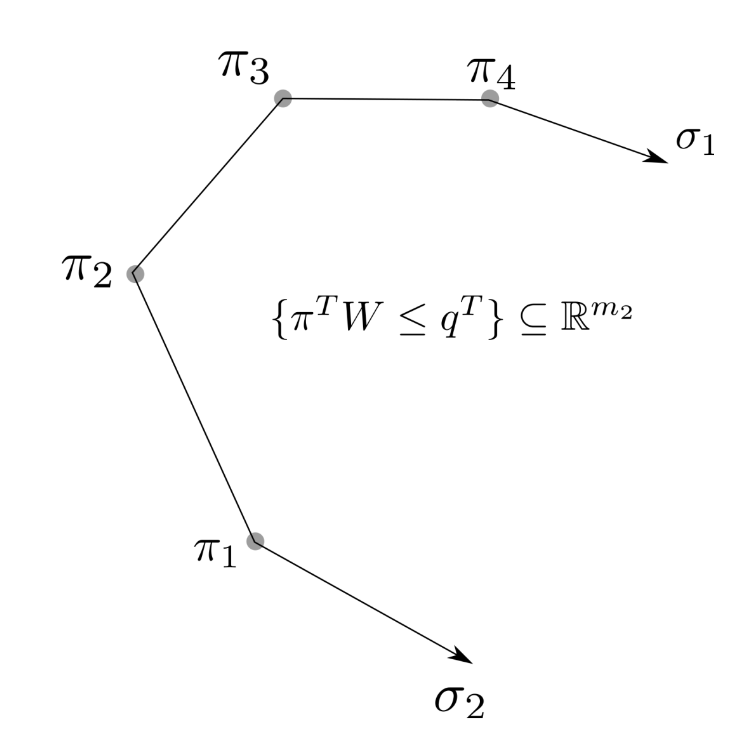
\includegraphics[width=.35\textwidth]{img/extreme.png}
\end{figure}
We can see that $V(x)$ is a piecewise linear convex function of $x$ and, defining $\pi_0$ as the dual optimal multiplier of \eqref{eq:benders} given $x_0$, then $\pi_0^T(h-Tx_0)$ is a supporting hyperplane of $V(x)$ at $x_0$, because it belongs to the subdifferential of $V(x)$ at $h-Tx_0$.
\begin{figure}[H]
	\centering
	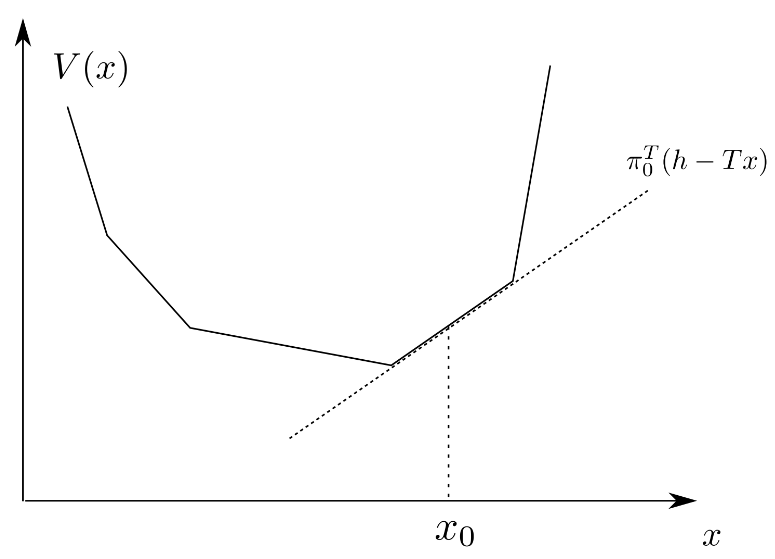
\includegraphics[width=.5\textwidth]{img/supporting_hyperplane.png}
\end{figure}
From this, we can also express the domain of $V$ as follows:
\begin{equation}
	dom(V) = \{x\ |\ \sigma^T(h-Tx)\le 0,\ \sigma\in R\}
\end{equation}
where $\sigma\in R$ is the set of extreme rays of $\pi^TW\le q^T$.
\begin{itemize}
	\item [$\to$] Note: when a domain is unbounded in a direction that does not improve the objective value, it is not a problem to its resolution.
\end{itemize}
\subsection{Reformulation}
The objective of the reformulation is to find a general form for the algorithm. That way, each iteration simply adds constraints of the same form, involving the minimum number of changes to the problem.
\begin{equation}
	\begin{aligned}
		&\min c^Tx + \theta \\
		&Ax=b\\
		&\sigma_r^T(h-Tx)\le0\quad \sigma_r\in R\\
		&\theta \ge \pi_e^T(h-Tx)\quad \pi_e\in E\\
		&x\ge0 
 	\end{aligned}
\end{equation}
where $\theta$ is a free variable.\\
The idea is to relax some inequalities that define $V(x)$ and $dom\ V$:\\
\begin{minipage}{.5\textwidth}
	\begin{equation}
		\begin{aligned}
			(M): \ \ & z_k = \min c^Tx+\theta\\
			& Ax= b\\
			&\sigma_r^T(h-Tx)\le0\quad \sigma_r\in R_k\subseteq R\\
			&\theta \ge \pi_e^T(h-Tx)\quad \pi_e\in E_k\subseteq E\\
			&x\ge0 
		\end{aligned}
	\end{equation}
\end{minipage}
\begin{minipage}{.5\textwidth}
	\begin{equation}
		\begin{aligned}
			(S): \ \ & V(\bar x) = \min_{x,y} q^Ty\\
			& Wy=h-Tx\\
			&x = \bar x\\
			&y\ge 0
		\end{aligned}
	\end{equation}
\end{minipage}
The solution of the main problem (M) above provides:
\begin{itemize}
	\item A lower bound $z_k\le z^\star$;
	\item A candidate solution $x_k$;
	\item An under-estimator of $V(x_k)$, $\theta_k \le V(x_k)$.
\end{itemize}
The solution of the subproblem (S) with input $x_k$ provides:
\begin{itemize}
	\item An upper bound $c^Tx_k+q^Ty_{k+1}\ge z^\star$;
	\item A new vertex $\pi_{k+1}$ or a new extreme ray $\sigma_{k+1}$.
\end{itemize}
\begin{figure}[H]
	\centering
	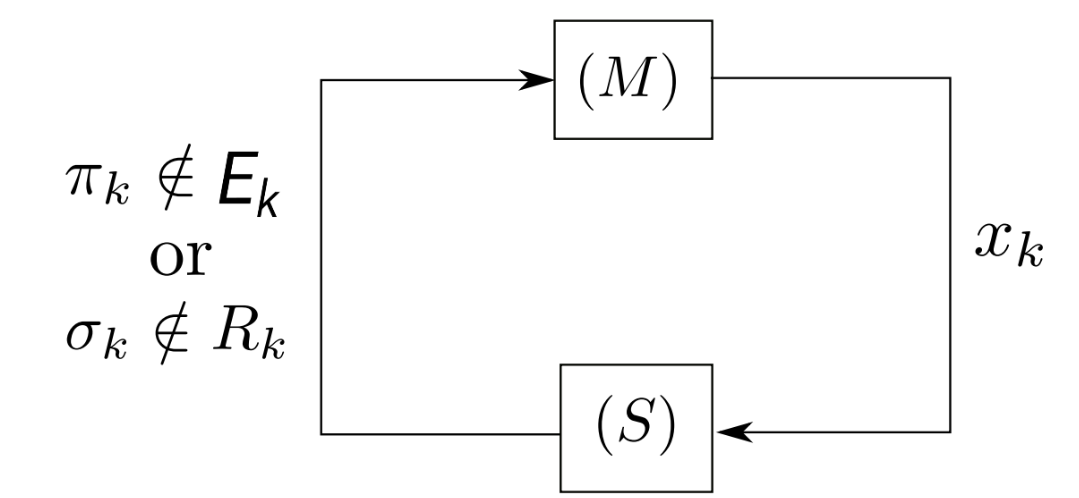
\includegraphics[width=.4\textwidth]{img/reformulation.png}
\end{figure}
In addition to the two problems defined above, we have the dual of (S):
\begin{equation}
	\begin{aligned}
		(D) \ : \ & \max_{\pi,\lambda} \lambda^Tx + \pi^Th
		& \pi^TW\le q^T\\
		& \pi^T T + \lambda = 0
	\end{aligned}
\end{equation}
With this, the formulation of the optimality cut becomes 
\begin{equation}
	\theta \ge \lambda^T(x-\bar x) + V(\bar x)
\end{equation}
\section{Benders Decomposition Algorithm}
\begin{algorithm}
	\caption{Benders Decomposition Algorithm}
	\begin{algorithmic}[1]
		\State \textbf{Step 0:} Set $k=0$, $E_0=R_0=\emptyset$;
		\State \textbf{Step 1:} Solve (M);
		\If {(M) is feasible}
		\State Store $x_k$;
		\Else \State break;\EndIf
		\State \textbf{Step 2:} Solve (S) (or (D)) with $x_k$ as input;
		\If {(S) is infeasible}
		\State Let $R_{k+1} = R_k\cup \{\sigma_{k+1}\}$;
		\State $k\gets k+1$;
		\Else \State Let $E_{k+1} = E_k \cup \{\pi_{k+1}\}$;
		\If {$E_{k+1} = E_k$} \State terminate with $(x_k,y_{k+1})$ as optimal solution;
		\Else \State Let $k\gets k+1$ and back to step 1.
		\EndIf 
		\EndIf 
	\end{algorithmic}
\end{algorithm}
\begin{itemize}
	\item [$\to$] Note: The algorithm takes finite time, as $E$ and $R$ are finite. 
\end{itemize}
\chapter{The L-Shaped Method}
For this resolution method, we start from the extensive form of the two-stage stochastic linear program:
\begin{equation}\label{eq:EF}
    \begin{aligned}
        &\min c^T x + \E_\omega[q(\omega)^T y(\omega)]\\
        &Ax = b\\
        &T(\omega)x + W(\omega)y(\omega) = h(\omega)\\
        &x\ge 0,y\ge 0\\
    \end{aligned}
\end{equation}
\section{Complete recourse}
In order to define the concept of recourse, we need the following sets:
\begin{itemize}
    \item $K_1 = \{x\ : \ Ax=b,x\ge 0\}$;
    \item $K_2 (\omega) = \{x\ : \ \exists y ,T_\omega x + W_\omega y = h_\omega,y\ge 0\}$;
    \item $K_2 = dom(V)\equiv \{x \ | \ V(x)<\infty\}$;
    \item if $\Omega$ is discrete, $K_2 = \cap_{\omega\in \Omega}K_2(\omega)$.
\end{itemize}
Relative complete recourse is when obeying the first-stage constraints ($Ax=b$) ensures that some feasible second-stage decisions exist, i.e. $K_1\subseteq K_2$.\\
Complete recourse is when a feasible second-stage decision exists, regardless of the first-stage decision and realization of uncertainty, i.e.
\begin{equation}
    \exists y\ge 0\text{ s.t. }Wy=t, \ \forall t\in \R^{m_2} \Longleftrightarrow \textcolor{red}{pos} W=\R^{m_2}
\end{equation}
\section{Value function}
Here, the second-stage value function and its dual are \\
\begin{minipage}{.5\textwidth}
    \begin{equation}\label{eq:Sw}
        \begin{aligned}
            (S_\omega): \ &Q_\omega(x) = \min_y q^T_\omega y\\
            & W_\omega y=h_\omega - T_\omega x\\
            & y\ge 0
        \end{aligned}
    \end{equation}
\end{minipage} 
\begin{minipage}{.5\textwidth}
    \begin{equation}
        \begin{aligned}
            (D_\omega)\ : \ &\max_\pi \pi^T (h_\omega-T_\omega x)\\
            & \pi^TW_\omega \le q^T_\omega 
        \end{aligned}
    \end{equation}
\end{minipage} 
and thus the expected value function is $V(x) = \sum_{\omega = 1}^N p_\omega Q_\omega (x)$, from which we can define the following problem
\begin{equation}
	\begin{aligned}
		(S) \ : \ & \min_y \sum_{\omega = 1}^N p_\omega q_\omega^Ty_\omega \\
		& Wy=h-Tx\\
		& y\ge 0
	\end{aligned}
\end{equation}
where $y$ and $h$ are the vectors of the $y_i,h_i$, and $T,W$ are the diagonal matrices of the $T_\omega,W_\omega$. 
\subsection{Properties}
Given a $x_0$, we denote $\pi_{\omega0}$ the dual optimal multipliers.
\begin{itemize}
    \item $V(x)$ and $Q_\omega(x)$ are piecewise linear convex functions of $x$;
    \item $\pi_{\omega0}^T(h_\omega-T_\omega x)$ is a supporting hyperplane of $Q_\omega(x)$ at $x_0$;
    \item $\sum_{\omega =1}^N p_\omega\pi_{\omega0}^T(h_\omega-T_\omega x)$ is a supporting hyperplane of $V(x)$ at $x_0$.
\end{itemize}
We denote $E$ the set of extreme points of $\{\pi:\pi^TW\le q^T\}$ and $R$ its set of extreme rays, while $E_\omega$ is the set of extreme points of $\{\pi:\pi^TW_\omega \le q_\omega^T\}$ and $R_\omega$ its set of extreme rays. \\
\subsection{Deterministic version}
The original problem \eqref{eq:EF} can be written as a deterministic equivalent program:
\begin{equation}\label{eq:M}
	\begin{aligned}
		(M)\ : \ &z_k = \min c^T_x+\theta \\
		& Ax=b\\
		& \sigma^T (p\cdot (h-Tx))\le 0,\sigma\in R_k \subseteq R\\
		&\theta \ge \pi^T (p\cdot (h-Tx)), \pi\in E_k \subseteq E \\
		&x\ge 0
	\end{aligned}
\end{equation}
where $p^T = (p_1\mathbb{1}_{n_2}^T, \cdot, p_N\mathbb{1}_{n_2}^T)$ and $\cdot$ is the componentwise product. The $\theta$ inequality can also be written in the following form:
\begin{equation}\label{eq:cut}
	\theta \ge \sum_{\omega = 1}^N p_\omega \pi_\omega^T (h_\omega-T_\omega x)
\end{equation}
Our main problem to solve is now this deterministic version, where the $\sigma$ inequalities are feasibility cuts, and the $\pi$ inequalities are the optimality cuts. 
\begin{figure}[H]
	\centering 
	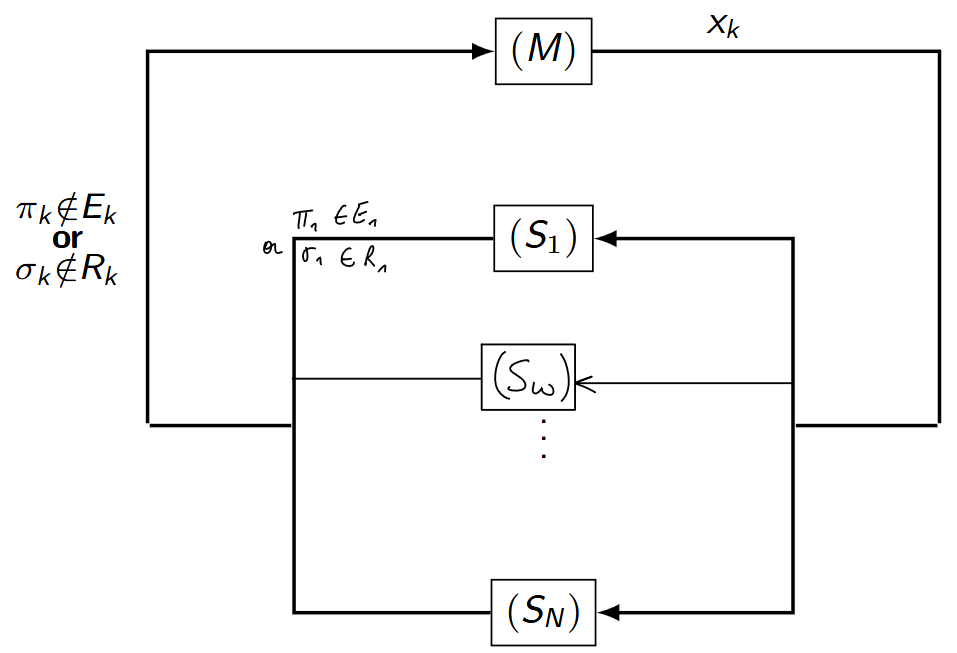
\includegraphics[width=.5\textwidth]{img/cuts.png}
\end{figure}
The goal of these cuts are to provide bounds on the solution of problem \eqref{eq:EF}. \\
\section{Bounds}
\begin{itemize}
	\item The solution of the main problem \eqref{eq:M} provides the following:
	\begin{itemize}
		\item A lower bound $z_k\le z^\star$;
		\item A candidate solution $x_k$;
		\item An under-estimator $\theta_k \le V(x_k)$;
	\end{itemize}
	\item The solution of all problems $(S_\omega)$ \eqref{eq:Sw} with the input $x_k$ provides the following:
	\begin{itemize}
		\item An upper bound $c^Tx_k + \sum_{\omega = 1}^N p_\omega q_\omega^Ty_{\omega, k+1}\ge z^\star$;
		\item A new vertex $\pi_{k+1}=(\pi^T_{1,k+1},\dots, \pi^T_{N,k+1})$ or a new extreme ray $\sigma_{k+1}=(0,\dots,\sigma_\omega^T,\dots,0)$. 
	\end{itemize}
\end{itemize}
\section{Final Algorithm}
\begin{algorithm}[H]
	\caption{The L-Shaped Algorithm}
	\label{algo:lshaped}
	\begin{algorithmic}[1]
		\State \textbf{Step 0:} Set $k=0$, $V_0 = R_0 = \emptyset$;
		\State \textbf{Step 1:} Solve $(M)$;
		\If{$(M)$ is feasible} \State Store $x_k$;
		\Else \State exit: infeasible;
		\EndIf
		\State \textbf{Step 2:} For $\omega=1,\dots,N$, solve $(S_\omega)$ with $x_k$ as input
		\If {$(S_\omega)$ is infeasible} \State $R_{k+1}\coloneqq R_k \cup \{\sigma_{k+1}\}$, where $\sigma_{k+1}$ is an extreme ray of $(S_\omega)$;
		\State $k\coloneqq k+1$;
		\State Go back to \textbf{Step 1}.
		\Else \State Store $\pi_{\omega,k+1}$;
		\EndIf 
		\State \textbf{Step 3:} $E_{k+1} = E_k \cup \{(\pi_{1,k+1}, \dots, \pi_{N,k+1})\}$;
		\If {$E_k = E_{k+1}$} \State Terminate with $(x_k,y_{k+1})$ as the optimal solution;
		\Else \State $k\coloneqq k+1$ and return to \textbf{Step 1}.
		\EndIf 
	\end{algorithmic}
\end{algorithm}
\section{Example}\label{sec:lshaped_example}
Let us do an example to better understand this algorithm. The initial problem is 
\begin{equation}
	\begin{aligned}
		&z = \min\E_\xi(y_1 + y_2)\\
		& \text{s.t. }0\le x\le 10\\
		& y_1-y_2 = \xi-x\\
		& y_1,y_2\ge 0\\
	\end{aligned}
\end{equation}
where we define 
\begin{equation}
	\xi = \begin{cases}
		1 & p_1 = 1/3\\
		2 & p_2 = 1/3\\
		4 & p_3 = 1/3\\
	\end{cases}
\end{equation}
The $\omega$ problems are \\
\begin{minipage}{.5\textwidth}
	\begin{equation}
		\begin{aligned}
			(S_\omega)\ : \ &\min y_1 + y_2 = |\xi-x|\\
			& y_1 - y_2 = \xi - x\\
			& y_1,y_2 \ge 0\\
		\end{aligned}
	\end{equation}
\end{minipage}
\begin{minipage}{.5\textwidth}
	\begin{equation}
		\begin{aligned}
			(D_\omega) \ : \ & \max_\pi \pi(\xi-x)\\
			&-1\le \pi\le 1
		\end{aligned}
	\end{equation}
\end{minipage}
The equality in the min can be added thanks to the definition of $(D_\omega)$.
\subsection{Iteration 1}
We start the algorithm with $x_1 = 0$. We first have to solve $(S_\omega)$ (or $(D_\omega)$), to get the value of $\pi$. We decide to solve $(D_\omega)$ because it is easier and gives us immediately the value of $\pi$. 
\begin{itemize}
	\item $\xi=1$ : $\pi^{(1)} = 1$;
	\item $\xi=2$ : $\pi^{(2)} = 1$;
	\item $\xi=4$ : $\pi^{(3)} = 1$;
\end{itemize}
And now we can find the cut using \eqref{eq:cut}, where $h_\omega - T_\omega x=\xi-x$ in this example. This gives as a first cut
\begin{equation}
	\theta \ge \frac{1}{3}\cdot 1 \cdot (1-x) + \frac{1}{3}\cdot 1 \cdot (2-x) + \frac{1}{3}\cdot 1 \cdot (4-x) = \frac{7}{3}-x
\end{equation}
To find the next value of $x$, the one we will use to start iteration 2, we try to minimize $V(x)$ under the constraints that $0\le x\le 10$ and $V(x) \ge \frac{7}{3}-x$, i.e. the cut. This gives us the new iterate: $x_2 = 10$. 
\subsection{Iteration 2}
We work in the same manner as we did in iteration 1, but this time using $x_2=10$. Solving once again $(D_\omega)$, we have 
\begin{itemize}
	\item $\xi = 1$: $\pi^{(1)} = -1$;
	\item $\xi = 2$: $\pi^{(2)} = -1$;
	\item $\xi = 4$: $\pi^{(3)} = -1$
\end{itemize}
As $h_\omega -T_\omega x= \xi-x$ still, the cut is now $\theta \ge x-\frac{7}{3}$.\\
To find $x_3$, we minimize $V(x)$ under the previous constraints, adding that $V(x) \ge x-\frac{7}{3}$. We find $x_3 = \frac{7}{3}$. 
\subsection{Iterations 3-4}
The two next iterations work in the same manner, and we find the two following cuts:
\begin{equation}
	\begin{aligned}
		&\theta \ge \frac{x+1}{3} \Longrightarrow x_4 = 1.5\\
		& \theta \ge \frac{5-x}{3} \Longrightarrow x_5 = 2\\
	\end{aligned}
\end{equation}
\subsection{Iteration 5}
At this iteration, we have $x_5=2$. As this value is optimal, no more iteration is needed.\textcolor{red}{How to show optimality?} Figure \ref{fig:l-shaped} illustrates the whole example. 
\begin{figure}
	\centering 
	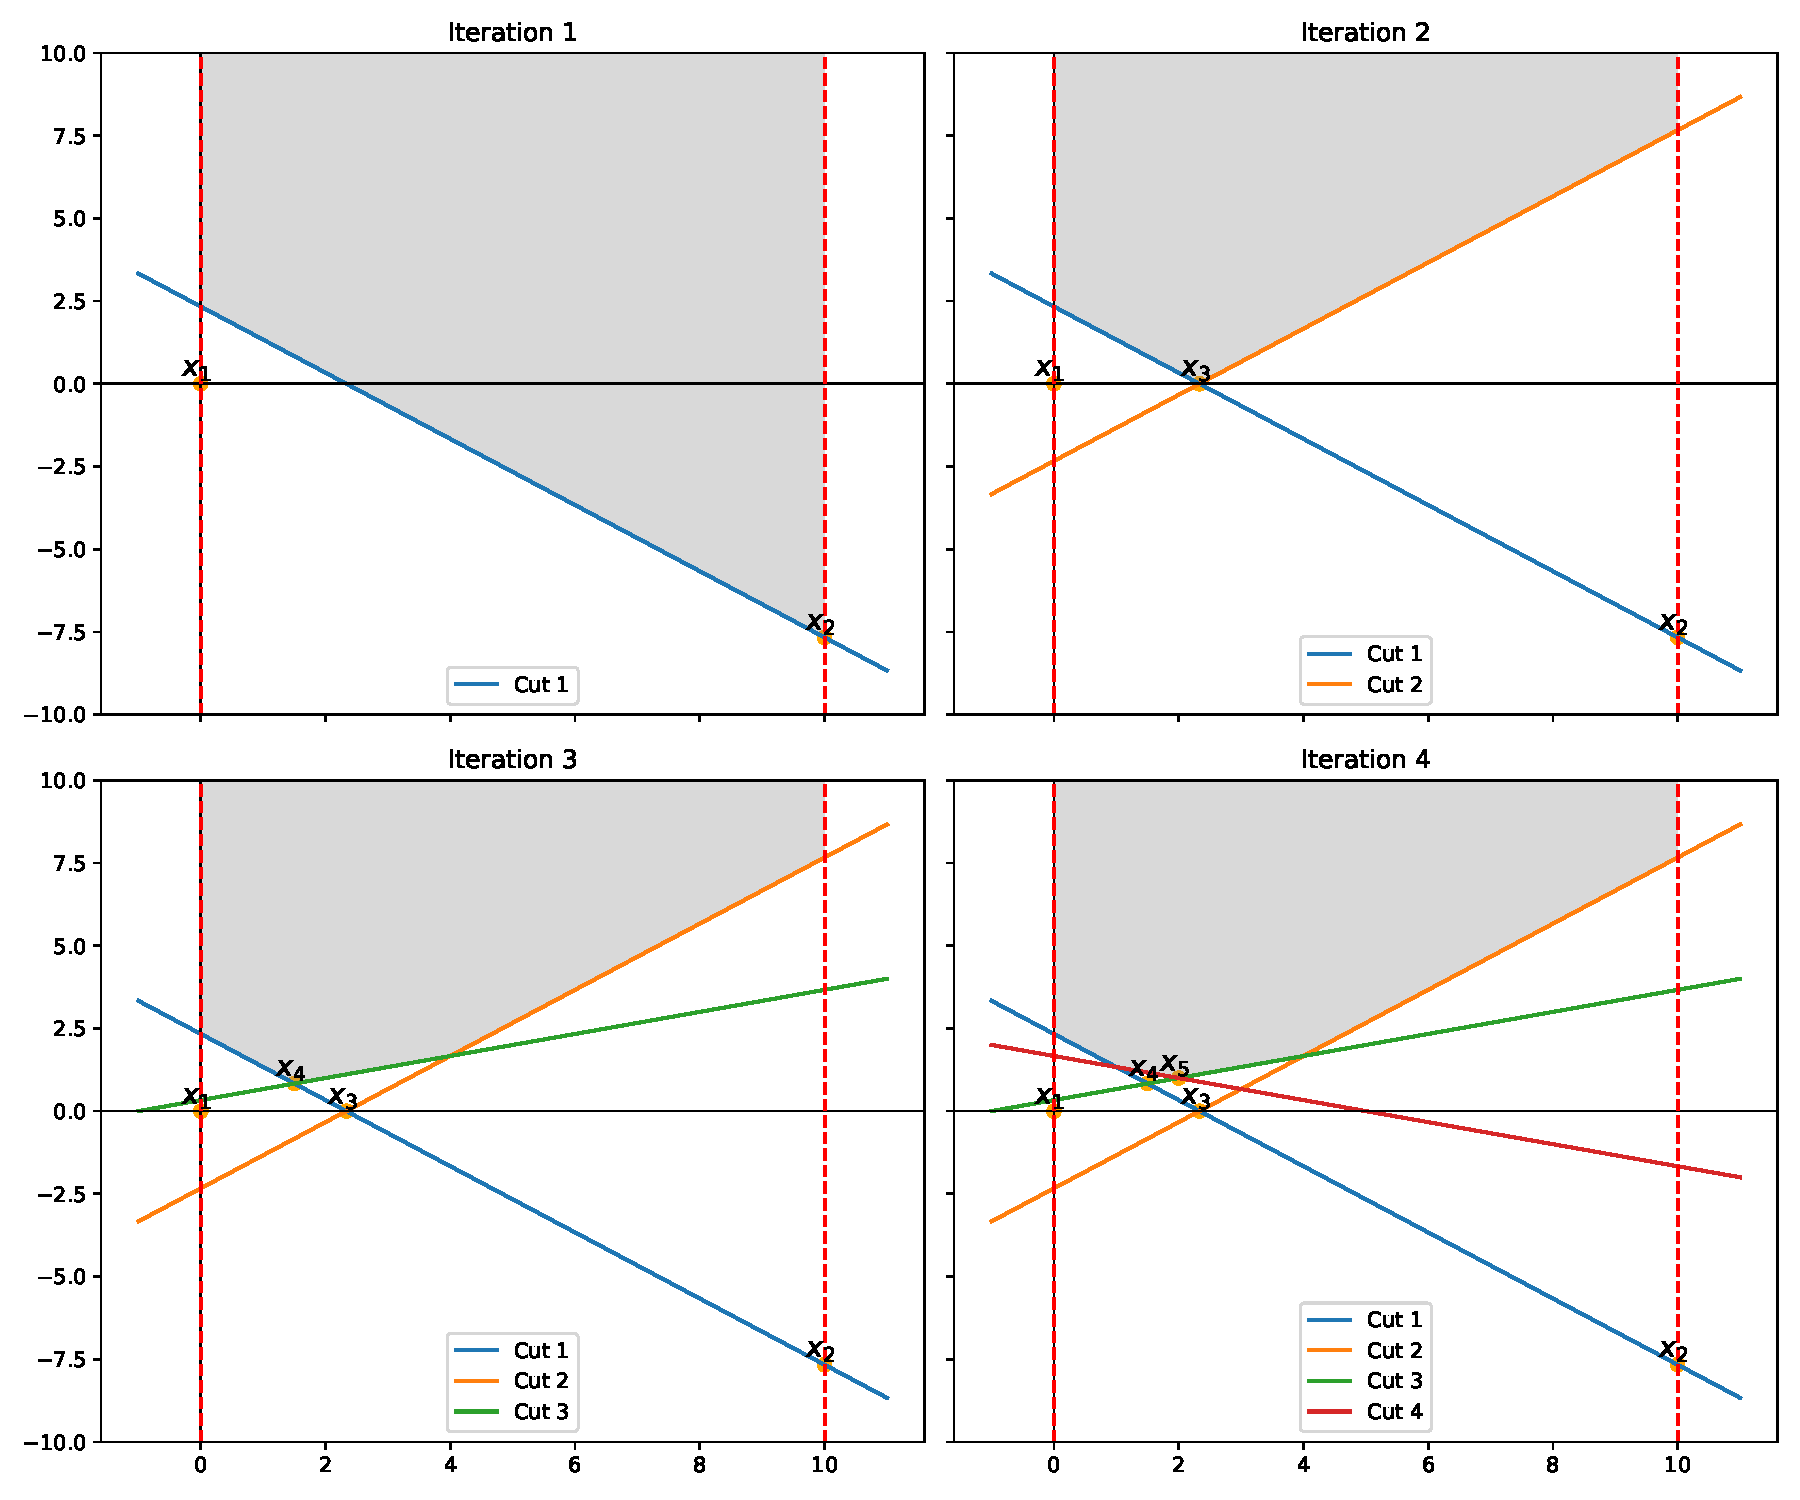
\includegraphics[width= .9\textwidth]{img/l_shaped_algo.pdf}
	\caption{L-Shaped Algorithm at each iteration}
	\label{fig:l-shaped}
\end{figure}
\chapter{The Multicut L-Shaped Method}
The idea of the multicut L-Shaped method is to do cuts as in the L-Shaped method, but on the $Q_\omega(x)$ instead of on the function $V(x)$ directly, and describe $V(x)$ from that. \\
As for the L-Shaped method, let us start from the extensive form of the 2-Stage stochastic linear program:
\begin{equation}
	\begin{aligned}
		\min& c^T x + \E_\omega[\min q(\omega)^Ty(\omega)]\\
		& Ax=b\\
		& T(\omega) x + W(\omega)y(\omega) = h(\omega)\\
		& x\ge0, y\ge 0
	\end{aligned}
\end{equation}
We know that 
\begin{equation}
	V(x) = \left\{\sum_\omega p_\omega \min q_\omega^T y_\omega | W_\omega y_\omega = h_\omega - T_\omega x ,y_\omega \ge 0\right\}
\end{equation}
\begin{equation}\label{eq:ssp}
	Q_\omega(x) = \left\{ \min q_\omega^T y|W_\omega y=h_\omega - T_\omega x, y\ge 0\right\}
\end{equation}
are piecewise linear functions of $x$, and the main problem corresponding to each function is the following:\\
\begin{minipage}{.5\textwidth}
	\begin{equation}
		\begin{aligned}
			z_k &= \min c^T x + \theta \\
			&Ax=b\\
			&\sigma^T(h-Tx)\le 0\quad \sigma\in R_k\subseteq R\\
			&\pi^T(h-Tx)\le \theta \quad \pi\in E_k\subseteq E\\
			& w\ge 0
		\end{aligned}
	\end{equation}
\end{minipage}
\begin{minipage}{.5\textwidth}
	\begin{equation}
		\begin{aligned}
			&\min c^Tx+\sum_\omega p_\omega \theta_\omega \\
			&Ax = b\\
			& \sigma^T(h_\omega-T_\omega x)\le 0\quad \sigma \in R_{\omega,k}\subseteq R_\omega\\
			& \pi^T(h_\omega-T_\omega x)\le \theta_\omega \quad \pi\in E_{\omega, k}\subseteq E_\omega\\
			& x\ge 0
		\end{aligned}
	\end{equation}
\end{minipage}
\section{Optimality cuts}
Let us consider a trial first-stage decision $x^v$, and $\pi_\omega$ the simplex multipliers of the second-stage problem \eqref{eq:ssp} (\textcolor{red}{what does that mean?}).\\
Then, $\sum_\omega p_\omega \pi_\omega^T(h_\omega - T_\omega x)$ supports $V(x)$ at $x^v$, and $\pi_\omega^T(h_\omega - T_\omega x)$ supports $Q_\omega(x)$ at $x^v$.\\
\begin{figure}
	\centering
	\begin{subfigure}[b]{0.49\textwidth}
		\centering
		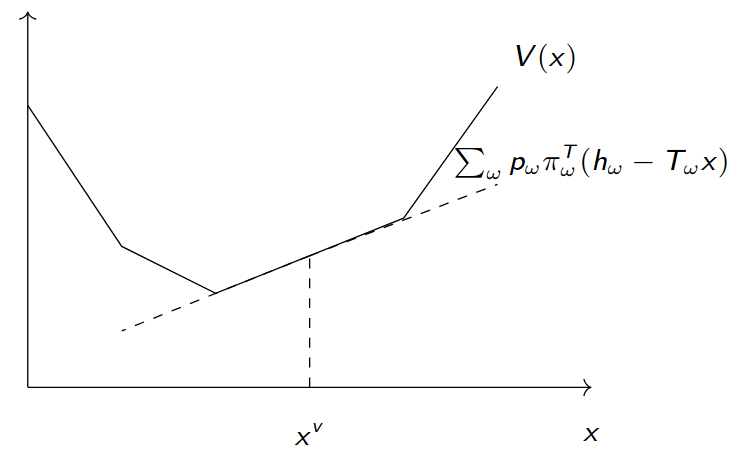
\includegraphics[width=\textwidth]{img/lshaped.png}
		\caption{Optimality cut for L-Shaped Method}
	\end{subfigure}
	\hfill 
	\begin{subfigure}[b]{0.49\textwidth}
		\centering
		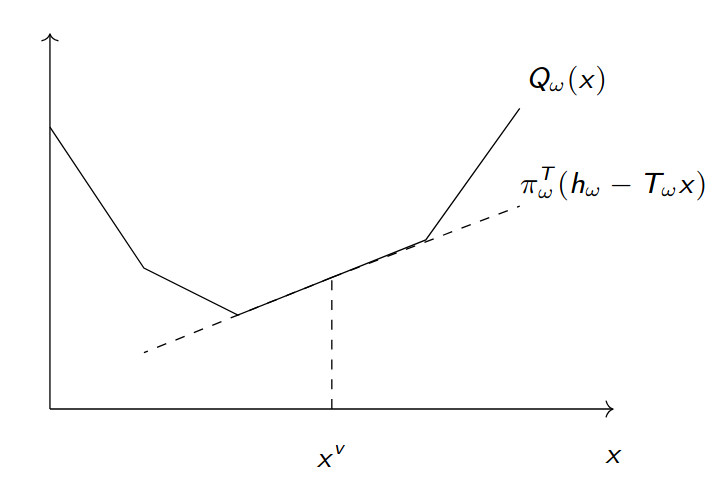
\includegraphics[width=\textwidth]{img/multicut.png}
		\caption{Optimality cut for Multicut L-Shaped Method}
	\end{subfigure}
\end{figure}
\begin{itemize}
	\item [$\to$] Note: The cuts of the multicut method are tigher than the L-Shaped method.
\end{itemize}
\section{Algorithm}
Here is the algorithm for the Multicut L-Shaped method, where the differences with the basic method are highlighted in green.
\begin{algorithm}[H]
	\caption{The Multicut L-Shaped Algorithm}
	\label{algo:multicut}
	\begin{algorithmic}[1]
		\State \textbf{Step 0:} Set $k=0$, \textcolor{green}{$E_{\omega,0} = R_{\omega,0}=$}$ \emptyset$;
		\State \textbf{Step 1:} Solve $(M)$;
		\If{$(M)$ is feasible} \State Store $x_k$;
		\Else \State exit: infeasible;
		\EndIf
		\State \textbf{Step 2:} For $\omega=1,\dots,N$, solve $(S_\omega)$ with $x_k$ as input
		\If {$(S_\omega)$ is infeasible}
		\State \textcolor{green}{$R_{\omega,k+1}\coloneqq R_{\omega, k} \cup \{\sigma_{\omega,k+1}\}$}, where $\sigma_{\omega, k+1}$ is an extreme ray of $(S_\omega)$;
		\State $k\coloneqq k+1$;
		\State Go back to \textbf{Step 1}.
		\Else \State Store $\pi_{\omega,k+1}$;
		\EndIf 
		\State \textbf{Step 3:} For $\omega=1,\dots,N$, let \textcolor{green}{$E_{\omega,k+1} = E_{\omega,k} \cup \{\pi_{\omega,k+1}\}$};
		\If {\textcolor{green}{$E_{\omega,k} = E_{\omega,k+1}$ for all $\omega$},} 
		\State Terminate with $(x_k,y_{k+1})$ as the optimal solution;
		\Else \State $k\coloneqq k+1$ and return to \textbf{Step 1}.
		\EndIf 
	\end{algorithmic}
\end{algorithm}
The algorithm is essentially the same as \ref{algo:lshaped}, with the difference that we solve a distinct problem for all $\omega$ instead of a global one. 
\section{Example}
Let us use the same problem as in last section (\ref{sec:lshaped_example}). 
\begin{equation}
	\begin{aligned}
		&z = \min\E_\xi(y_1 + y_2)\\
		& \text{s.t. }0\le x\le 10\\
		& y_1-y_2 = \xi-x\\
		& y_1,y_2\ge 0\\
	\end{aligned}
\end{equation}
where we define 
\begin{equation}
	\xi = \begin{cases}
		1 & p_1 = 1/3\\
		2 & p_2 = 1/3\\
		4 & p_3 = 1/3\\
	\end{cases}
\end{equation}
The main problem is 
\begin{equation}
	\begin{aligned}
		(M): & \ \min \sum_\omega \frac{1}{3}\theta_\omega\\
		& \theta_\omega \ge -10^6\\
		& 0\le x\le 10\\
	\end{aligned}
\end{equation}
And the subproblem and its dual are \\
\begin{minipage}{.5\textwidth}
	\begin{equation}
		\begin{aligned}
			(S_\omega)\ : \ &\min y_1 + y_2 = |\xi_\omega-x|\\
			& y_1 - y_2 = \xi_\omega - x\\
			& y_1,y_2 \ge 0\\
		\end{aligned}
	\end{equation}
\end{minipage}
\begin{minipage}{.5\textwidth}
	\begin{equation}\label{eq:dual}
		\begin{aligned}
			(D_\omega) \ : \ & \max_{\pi_\omega} \pi_\omega(\xi_\omega-x)\\
			&-1\le \pi_\omega \le 1
		\end{aligned}
	\end{equation}
\end{minipage}
\begin{itemize}
	\item [$\to$] Note: the bound $\theta_\omega \ge -10^6$ is needed for the first iteration but is not really a restriction. 
\end{itemize}
\subsection{Iteration 1}
At the first iteration, we solve problem (M) for $x$. The solution is \textcolor{red}{$x_1=0$}, and this value is used to solve problem \eqref{eq:dual}. The solution for $\pi$ is 1 for each $\xi_\omega$ and so we add the cuts 
\color{red}
\begin{equation}
	\theta_\omega \ge \xi_\omega -x \Longrightarrow \begin{cases}
		\theta_1 \ge 1-x\\
		\theta_2 \ge 2-x\\
		\theta_3 \ge 4-x\\
	\end{cases}\color{black}
\end{equation}\color{black}
We add this to the main problem (M) for the next iteration.
\subsection{Iteration 2}
We now have a problem with 5 constraints. The new problem is 
\begin{equation}
	\begin{aligned}
		& \min \sum_\omega \frac{1}{3}\theta_\omega \\
		& \theta_\omega \ge -10^{6}\\
		& 0\le x\le 10\\
		& \color{red}\theta_\omega \ge \xi_\omega -x \quad \forall \omega=1,2,3\color{black}
	\end{aligned}
\end{equation}
We solve for $x$ and find \textcolor{green}{$x_2=10$}. We can solve problem $(D_\omega)$ with this value as input, and the solution is $\pi_\omega = -1$ for each value of $\omega$. Once again, we add those constraints to the main problem:
\begin{equation}
	\color{green}
	\theta_\omega \ge x-\xi_\omega \Longrightarrow \begin{cases}
		\theta_1 \ge x-1\\
		\theta_2 \ge x-2\\
		\theta_3 \ge x-3
	\end{cases}\color{black}
\end{equation}
\subsection{Iteration 3}
We can now formulate the problem for this next iteration:
\begin{equation}
	\begin{aligned}
		&\min \sum_\omega \frac{1}{3}\theta_\omega \\
		\theta_\omega &\ge -10^6\\
		0&\le x\le 10\\
		\color{red} \theta_\omega &\color{red}\ge \xi_\omega-x\\
		\color{green}\theta_\omega &\color{green} \ge x-\xi_\omega \color{black}
	\end{aligned}
\end{equation}
Solving for $x$, \textcolor{blue}{$x_3=2$}. Solving now $(D_\omega)$, the constraints to be added are the following:
\begin{equation}
	\color{blue}
	\begin{cases}
		\pi_1 =-1  \Rightarrow \theta_1 \ge x-1 \\
		\pi_2 = [-1,1] \Rightarrow \theta_2 \ge x-2\\
		\pi_3 = 1 \Rightarrow \theta_3 \ge 4-x\\
	\end{cases}\color{black}
\end{equation}
Note that the constraint for $\theta_2$ is arbitrary as $\pi_2$ can take any value. However, as we already have the constraints $\theta_2 \ge x-2$ and $\theta_2\ge 2-x$, any value of $\pi_2\in [-1,1]$ is a linear combination of the two. As we have only added constraints that already existed, we already know that $x_4$ will have the same value as $x_3$, and so we have converged to the optimal solution. The other method to check convergence is to have a lower bound and upper bound with the same value. 
\section{Pros and Cons}
The Multicut L-Shaped method has a more detailed description of the value function $V(x)$ thanks to the separation in several terms $Q_\omega(x)$, but the main problem is bigger as we add $N$ constraints at each iteration instead of $1$. Typically, fewer iterations are required in the Multicut, but each iteration takes more time. 
\chapter{Nested Decomposition}
\section{Backward Solution of Multistage Stochastic Linear Programs}
Let us remember the terminology of scenario trees in \ref{sec:st}. We have already mentionned that we can use dynamic programming to solve the problem in scenario tree formulation. The method consists in computing recursively the values of $Q_\omega$ and $V_\omega$:\\
\begin{equation}
	\begin{aligned}
		Q_t(x_{t-1},\xi_t) &= \min_{x_t} c_t(\omega_{[t]})^T x_t + V_{t+1} (x_t, \omega_{[t]})\\
		& T_{t-1}(\omega_{[t]})x_{t-1} + W_t(\omega_{[t]})x_t = h_t(\omega_{[t]})\\
		& x_t\ge 0\\
		V_t(x_{t-1}, \omega_{[t-1]}) &= \E_{\xi_t} [Q_t(x_{t-1}, \xi_t)|\omega_{[t-1]}]
	\end{aligned}
\end{equation}
We formulate the problems starting from $t=H$ and go back to $t=1$, where we can solve with no previous step. From this, we go back increasing $t$ to solve each step. The initial step $t=1$ is 
\begin{equation}
	\begin{aligned}
		\min \ & c_1^Tx_1 \\
		&W_1x_1=h_1\\
		&x_1\ge 0
	\end{aligned}
\end{equation}
As usual, $V_{t+1, \omega_{[t]}}$ and $Q_{t+1}(x_t, \xi_{t+1})$ are piecewise linear and convex, and their domain are polyhedral. 
\section{Nested L-Shaped Decomposition Subproblem}
We have already seen how to solve a two-stage stochastic program (L-shaped or multicut). For more than 2 stages, we need to decompose the problem. 
\begin{itemize}
	\item [$\to$] Note: we will use indices. The first index denotes time and the second denotes the scenario.
\end{itemize}
\subsection{NLDS}
The idea is to decompose into smaller and deterministic linear programs as shown on \ref{fig:nested}.
\begin{figure}[H]
	\centering 
	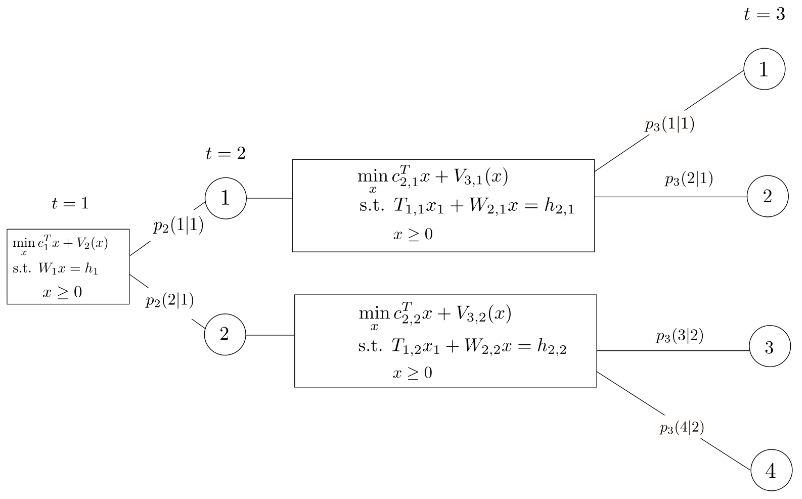
\includegraphics[width=.7\textwidth]{img/nested.png}
	\caption{Idea of Nested Decomposition}
	\label{fig:nested}
\end{figure}
The building blocks are the Nested L-Shaped Decomposition Subproblems (NLDS$(t,k)$), the problems at stage $t$ and scenario $k$. Solving each blocks gives information to the previous and also the next blocks: the algorithm is recursive in both direction. 
\begin{figure}[H]
	\centering 
	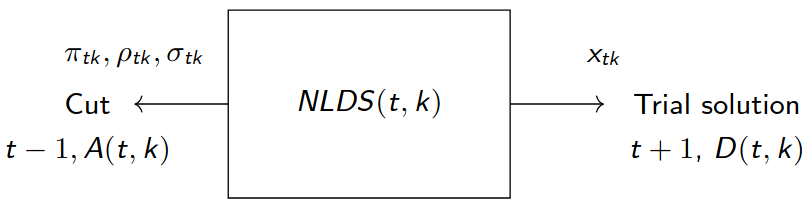
\includegraphics[width=.7\textwidth]{img/NLDS.png}
	\caption{Building block - NLDS($t,k$)}
\end{figure}
where $A(t,k)$ is the ancestor of outcome $k$ in period $t$, and $D(t,k)$ are the descendants of outcome $k$ at period $t$. \\
For each stage $t=1,\dots,H-1$ and each scenario $k=1,\dots,|\Xi_{[t]}|$, the problem is 
\begin{equation}
	\begin{aligned}
		NLDS(t,k): \ &\min_{x,\theta} (c_{t,k})^Tx+\theta \\
		(\pi) \quad & W_{t,k}x = h_{t,k}-T_{t-1,k}x_{t-1, A(t,k)} \\
		(\rho_j) \quad & E_{t,k,j}x + \theta \ge e_{t,k,j} \qquad j=1, \dots r_{t,k} \qquad \text{Optimality cut}\\
		(\sigma_j) \quad & D_{t,k,j} x\ge d_{t,k,j}\qquad j=1,\dots, s_{t,k} \qquad \quad \text{Feasibility cut}\\
		&x\ge 0
	\end{aligned}
\end{equation}
where $\Xi_{[t]}$ is the support of $\xi_{[t]}$, $A(t,k)$ is the ancestor of the realization $k$ at stage $t$, and $x_{t-1, A(t,k)}$ is the current solution from $A(t,k)$. 
\subsection{Boundary conditions}
To be able to finish the recursivity at $t=1$ and $t=H$, we need boundary conditions. 
\begin{itemize}
	\item For $t=1$, $h_{t,k}-T_{t-1, k}x_{t-1, A(t,k)}$ is replaced by a value $b$;
	\item For $t=H$, $\theta$ and the feasibility and optimality constraints are removed.
\end{itemize}
\subsection{Dual of NLDS}
The dual problem of NLDS$(t,k)$ is 
\begin{equation}\label{eq:dual-nlds}
	\begin{aligned}
		\max_{\pi,\rho,\sigma}&\ \textcolor{blue}{\pi^T(h_{t,k} - T_{t-1,k}x_{t-1, A(t,k)}) + \sum_{j=1}^{s_{t,k}} \sigma_j^T d_{t,k,j}}+ \sum_{j=1}^{r_{t,k}} \rho_j^T e_{t,k}\\
		& \textcolor{violet}{\pi^T W_{t,k} + \sum_{j=1}^{s_{t,k}} \sigma_j^T D_{t,k,j}} + \sum_{j=1}^{r_{t,k}} \rho_j^T E_{t,k,j} \le c_{t,k}^T\\
		& \sum_{j=1}^{r_{t,k}} \mathbb{1}^T \rho_j = 1\\
		&\rho, \sigma \ge 0
	\end{aligned}
\end{equation}
\section{Cuts}
\subsection{Feasibility cuts}
If NLDS$(t,k)$ is infeasible, the solver returns a set $(\pi, \sigma_1, \dots, \sigma_{s_{t,k}})$ with $\sigma_j \ge 0$ such that 
\begin{itemize}
	\item the blue term in \eqref{eq:dual-nlds} is strictly positive;
	\item the violet term in \eqref{eq:dual-nlds} is nonpositive.
\end{itemize}
This gives the following feasibility cut for NLDS$(t-1, a(k))$
\begin{equation}
	D_{t-1, A(t,k)} x\le d_{t-1, A(t,k)} \qquad \text{where} \qquad \begin{cases}
		D_{t-1, A(t,k)} = \pi^T T_{t-1,k}\\
		d_{t-1, A(t,k)} = \pi^Th_{t,k} +\sum_{j=1}^{s_{t,k}} \sigma_j^T d_{t,k,j}
	\end{cases}
\end{equation}
\subsection{Optimality cuts}
After solving NLDS$(t,k)$ for all $k\in D_{t-1,j}$, we can compute the cut with the following parameters:
\begin{equation}
	\begin{aligned}
		E_{t-1,j} &= \sum_k p_t(k|j) \cdot \pi_{t,k}^T T_{t-1,k}\\
		e_{t-1,j} &= \sum_k \left[p_t(k|j)\cdot \left(\pi_{t,k}^Th_{t,k} + \sum_{i=1}^{r_{t,k}} \rho_{t,k,i}e_{t,k,i} + \sum_{i=1}^{s_{t,k}} \sigma_{t,k,i}^Td_{t,k,i}\right)\right]
	\end{aligned}
\end{equation}
From which we find an optimality cut for NLDS$(t-1,j)$:
\begin{equation}
	E_{t-1,j}x+\theta \ge e_{t-1,j}
\end{equation}
\textcolor{red}{To what does the set $D_{t-1,j}$ correspond?} 
\begin{itemize}
	\item [$\to$] Note: If all sets $\Xi_{[t]}$ are finite and all $x$ have finite upper bounds, then the nested L-shaped method converges to an optimal solution in a finite number of iterations.
\end{itemize}
\subsection{Direction of movement}
Whenever we solve one NLDS$(t,k)$, some data is generated:
\begin{itemize}
	\item If the problem is feasible:
	\begin{itemize}
		\item The trial decision $x_{t,k}$ that can be sent forward;
		\item An optimality cut that can be sent backwards;
	\end{itemize}
	\item If infeasible, a feasibility cut that can be sent backwards.
\end{itemize}
There exist several ways to move in the algorithm. Here are three of them:
\begin{itemize}
	\item Fast-forward-fast-back: move in the current direction as far as possible;
	\item Fast-forward: move forward whenever it is possible;
	\item Fast-back: move backwards whenever it is possible.
\end{itemize}
\section{Example}\label{sec:example_nlds}
The problem we want to solve here is the following:
\begin{equation}
	\begin{aligned}
		\min &10x_1 + \E[15x_2+20x_3]\\
		& x_1+x_2\ge \xi_2\\
		& x_2+x_3\ge \xi_3\\
		& x_i \ge 0
	\end{aligned}
\end{equation}
where 
\begin{equation}
	\xi_2 = \begin{cases}
		40\ \text{w. p. } 1/2\\
		60\ \text{w. p. }1/2\\
	\end{cases}
	\qquad \xi_3 = \begin{cases}
		20\ \text{w. p. }1/2\\
		30\ \text{w. p. }1/2
	\end{cases}
\end{equation}
The sets defining the problems are the following\\
\begin{minipage}{.33\textwidth}
	\begin{equation}
		\begin{aligned}
			\Omega_1 &= \{I\}\\
			\Omega_2 &= \{40,60\}\\
			\Omega_3 &= \{20,30\}\\
			\Omega &= \times_{i=1}^3 \Omega_i
		\end{aligned}
	\end{equation}
\end{minipage}
\begin{minipage}{.33\textwidth}
	\begin{equation}
		\begin{aligned}
			S_1 &= \{1\}\\
			S_2 &= \{1,2\}\\
			S_3 &= \{1,2\}\\
		\end{aligned}
	\end{equation}
\end{minipage}
\begin{minipage}{.33\textwidth}
	\begin{equation}
		\begin{aligned}
			S_{[1]} &= \{1\}\\
			S_{[2]} &= \{(1,1), (1,2)\}\\
			S_{[3]} &= \{(1,1,1),(1,1,2), \dots\}\\
			S_{[t]} &= \times_{i=1}^t S_t
		\end{aligned}
	\end{equation}
\end{minipage}
Here is the tree we use to find the solution.
\begin{figure}[H]
    \centering 
    \resizebox{\textwidth}{!}{
    \begin{tikzpicture}[
        level 1/.style={sibling distance=8cm},
        level 2/.style={sibling distance=4cm},
        level distance=3cm,
        every node/.style={draw, rectangle split, rectangle split parts=2, align=center},
        edge from parent/.style={draw, ->}
        ]
        
        \node {\nodepart{one} NLDS$(1,1)$
        \nodepart{two} $\min 10x_1+\theta$\\ s.t. $x_1\ge0$\\$\theta\ge 0$}
        % First level
        child {node {\nodepart{one} NLDS$(2,1)$
        \nodepart{two} $\min 15x_2 + \theta$\\ s.t. $x_2 \ge40-x_1$\\ $x_2\ge 
        0$} 
        % Second level
        child {node {\nodepart{one} NLDS(3,1) \nodepart{two} $\min 20x_3$\\ s.t. $x_3 \ge 20-x_2$\\$ x_3\ge 0$}
        child {node {\nodepart{one} Dual \nodepart{two} $\max_\pi (20-x_2)\pi$\\ s.t. $0\le \pi\le 20$}}}
        child {node {\nodepart{one} NLDS(3,2) \nodepart{two} $\min 20x_3$\\ s.t. $x_3\ge 30-x_2$\\$ x_3\ge 0$}
        child {node {\nodepart{one} Dual \nodepart{two} $\max_\pi (30-x_2)\pi$\\ s.t. $0\le \pi\le 20$}}}
        }
        child {node {\nodepart{one} NLDS(2,2)
        \nodepart{two} $\min 15x_2+\theta$\\ s.t. $x_2 \ge 60-x_1$\\$ x_2\ge0$}
        child {node {\nodepart{one} NLDS(3,3) \nodepart{two} $\min 20x_3$\\ s.t. $x_3\ge 20-x_2 $\\$ x_3 \ge 0$}
        child {node {\nodepart{one} Dual \nodepart{two} $\max_\pi (20-x_2)\pi$\\ s.t. $0\le \pi\le 20$}}}
        child {node {\nodepart{one} NLDS(3,4) \nodepart{two} $\min 20x_3$\\ s.t. $x_3 \ge 30-x_2$\\$ x_3\ge0$}
        child {node {\nodepart{one} Dual \nodepart{two} $\max_\pi (30-x_2)\pi$\\ s.t. $0\le \pi\le 20$}}}
        };
    \end{tikzpicture}}
\end{figure}
\subsection{First pass}
We decide to use the FFFB method. 
\begin{enumerate}
	\item Solving NLDS(1,1), we get $x_1=0$, which we put in each subproblem NLDS$(2,\cdot)$. The probability to go in each scenario is 1/2. 
\end{enumerate}
\textcolor{red}{Continue the explanation when the example is clear. Take notes of someone else.}
\subsection{Algorithm on paper}
\begin{enumerate}
	\item Solve the subproblem of stage 1;
	\item For each stage $(t,k)$, solve the subproblem with the solution of $(t-1, a(k))$ as inputs;
	\item Solve the dual of the last stage to find the cut;
	\item The cut is $\theta \ge e_{t-1,j}-E_{t-1,j}x$ for each subproblem $j$, where \footnote{I don't know what the term in parentheses means in $e_{t-1,j}$ means but it is just $h_{t,k}$ in the first pass.}
	\begin{equation}
		\begin{aligned}
			E_{t-1,j} &= \sum_k p_t(k|j)\pi_{t,k}^T T_{t-1,k}\\
			e_{t-1,j} &= \sum_k \left[p_t(k|j)\left(\pi_{t,k}^T h_{t,k}+\sum_i \rho_i^T e_{t,k} + \sum_i \sigma_i^T p_{t,k,i}\right)\right]
		\end{aligned}
	\end{equation}
	\item Put the cut found in $(t,k)$ in the previous level $(t-1,a(k))$ and solve the dual of $(t-1,a(k))$ with all of its new constraints to find a cut for its own ancestor problem;
	\item Repeat until $t=1$;
	\item Go back to step 1.
\end{enumerate}
\chapter{Stochastic Dual Dynamic Programming}
\section{Motivation}
The nested decomposition requires a huge number of iterations: $\sum_{t=1}^{H-1}\prod_{j=1}^t|S_j|$ for the forward pass and $\sum_{t=2}^H \prod_{j=1}^t |S_j|$ for the backward pass. It is not feasible on practice as it will almost always overload the memory. The stochastic dual dynamic programming (SDDP) solves this issue by,
\begin{itemize}
	\item in the forward pass, simulating instead of enumerating, i.e. it takes some instead of all sample paths. This gives a probabilistic upper bound. 
	\item in the backward pass, sharing the cuts among the nodes of the same time period.
\end{itemize}
And this method can be done on a lattice, while the sharing cannot be done on the tree due to the structure (see \ref{fig:sharing}).
\begin{figure}[H]
	\centering 
	\begin{subfigure}[b]{.49\textwidth}
		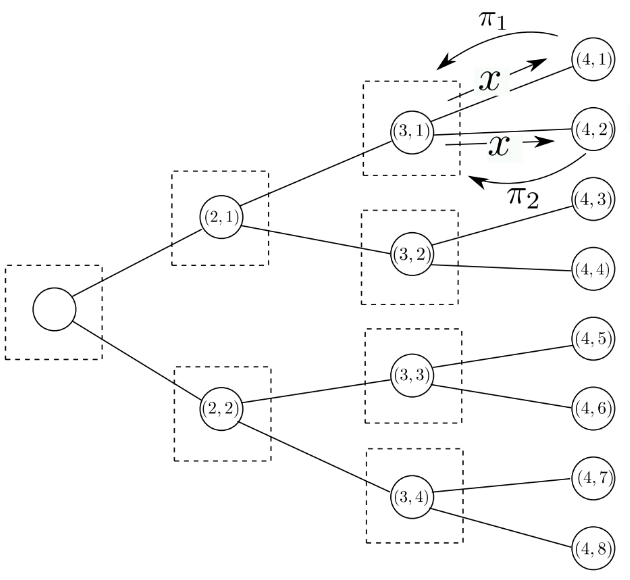
\includegraphics[width=\textwidth]{img/tree_no_sharing.png}
		\caption{Scenario tree without cut sharing.}
	\end{subfigure}
	\hfill 
	\begin{subfigure}[b]{.5\textwidth}
		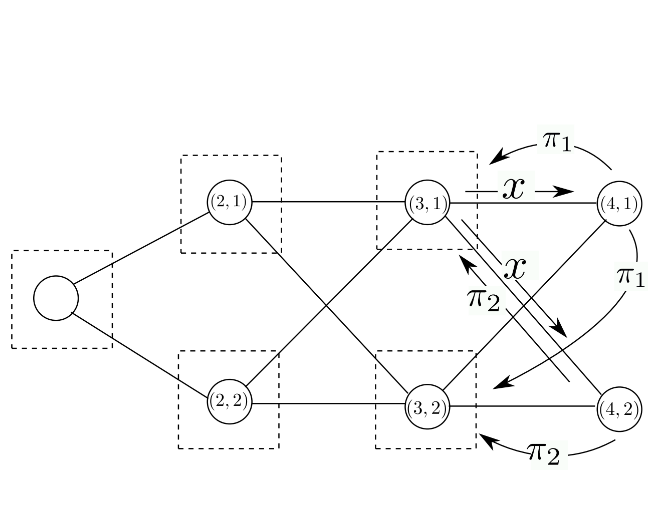
\includegraphics[width=\textwidth]{img/lattice_sharing.png}
		\caption{Cut sharing in a lattice.}
	\end{subfigure}
	\caption{The dashed boxes represent the storage of a different value function.}
	\label{fig:sharing}
\end{figure}
\begin{itemize}
	\item [$\to$] Note: in case of serial independence (cf. \ref{sec:serial_ind}), the values $\pi_i$ can simply be returned to the parent node of the same scenario as the problem is identical from $t$ onwards, independently of the node $k$ in stage $t$.
\end{itemize}
\section{SDDP}
The basic idea is to follow those 2 steps:
\begin{enumerate}
	\item Sampling: generate $K$ samples of random process $\{\xi_{1,i},\dots, \xi_{H,i}\}$ for $i=1,\dots, K$;
	\item Optimization: Solve NLDS in order to generate the trial decision variables $\hat x_{t,i}$:
	\begin{equation}
		\begin{aligned}
			\min\ & c_{t,k}^Tx+\theta\\
			& T_{t-1,k}\hat x_{t-1,i} + W_{t,k}x = h_{t,k}\\
			& E_{t,k}x+\theta \cdot \mathbb{1} \ge e_{t,k}\\
			&x\ge 0
		\end{aligned}
	\end{equation}
\end{enumerate}
At each forward pass, we solve $H-1$ NLDS problems, and so for $K$ samples of $\xi_{[H]}$, we solve $1+K\cdot (H-2)$ linear programs. \\
For the backward pass, for a given trial sequence $x_{[H]}$, we solve $\sum_{t=2}^H|\Xi_t|$ linear programs, and so for $K$ trial sequences, we solve $K\sum_{t=2}^H|\Xi_t|$ linear programs. 
\subsection{Algorithm}
\begin{algorithm}[H]
	\caption{SDDP}
	\label{algo:sddp}
	\begin{algorithmic}[1]
		\State \underline{Forward pass:}
		\State Solve NLDS(1) and let $x_1$ be the optimal solution. Initialize $\hat x_{1,i}=x_1$ for all $i=1,\dots,K$.
		\For{$t=2,\dots,H; i=1,\dots,K$}
		\State Sample an outcome $\xi_{t,i}$ from the set $\Xi_t$;
		\State Solve NLDS$(t,i)$ with trial decision $\hat x_{t-1, i}$;
		\State Store the optimal solution as $\hat x_{t,i}$.
		\EndFor
		\State \underline{Backward pass:}
		\For{$t=H, \dots,2$}
		\For{$i=1,\dots, K$}
		\For {$k=1,\dots, |\Xi_t|$}
		\State Solve NLDS$(t,k)$ using the trial decision $\hat x_{t-1,i}$
		\EndFor 
		\For {$j=1,\dots, |\Xi_{t-1}|$}
		\State Compute 
		\begin{equation}
			\begin{aligned}
				E_{t-1,j,i} &= \sum_{k=1}^{|\Xi_t|} p_t(k|j) \cdot \pi_{t,k,i}^T T_{t-1,k}\\
				e_{t-1,i,j} &= \sum_{k=1}^{|\Xi_t|} p_t(k|j)\cdot \left(\pi_{t,k,i}^Th_{t,k} + \rho_{t,k,i}e_{t,k}\right)
			\end{aligned}
		\end{equation}
		\EndFor
		\State Add this optimality cut to every NLDS$(t-1,j)$ for $j=1,\dots,|\Xi_{t-1}|$:
		\begin{equation}
			E_{t-1,j,i}x+\theta \ge e_{t-1,j,i}
		\end{equation}
		\EndFor
		\EndFor
		\State \textcolor{red}{There's an index problem somewhere i think.}
	\end{algorithmic}
\end{algorithm}
\begin{itemize}
	\item [$\to$] Note: the variables $(\pi_{t,k,i}, \rho_{t,k,i})$ are the dual multipliers generated by the trial $i$.
\end{itemize}
We can increase the number $K$ of forward samples to get a faster learning of the value function, but this requires to solve more LPs at each forward-backward pass, and the number of NLDS grows faster too. 
\subsection{Stop condition}
A good way to determine when to terminate SDDP is through the condition [lower bound] $\approx$ [upper bound]. 
\begin{itemize}
	\item The lower bound is found through the objective function value of NLDS(1) since that problem finds an underestimate of $V_2(x)$ on a superset of the domain of $V_2(x)$;
	\item The upper bound is probabilistic and found with the algorithm. 
\end{itemize}
\subsubsection{Upper bound}
Suppose that we draw a sample $i$ of $\xi_{[H]}$ and perform a forward pass. This gives a vector $\hat x_{t,i}$, $t=1,\dots,H$, and we can compute the cost $z_i = \sum_{t=1}^{H} c_{t,i}\hat x_{t,i}$. Repeating this $K$ times, we get a distribution of i.i.d. costs $z_i$.\\
By the Central Limit Theorem, $\bar z = \frac{1}{K}\sum_{i=1}^Kz_i$ converges to a Gaussian with standard deviation estimated by 
\begin{equation}
	\sigma = \sqrt{\frac{1}{K^2} \sum_{k=1}^K (\bar z-z_i)^2}
\end{equation}
Note that each sequence $\hat x_{[H]}$ is feasible, but not necessarily optimal, and so $\bar z$ is an estimate of an upper bound. \\

We usually consider that we can terminate if $\underline{z}\in (\bar z-2\sigma, \bar z+2\sigma)$, which is the 95.4\% confidence interval of $\bar z$. 
\subsubsection{Choosing \texorpdfstring{$K$}{}}
To ensure an optimality gap of 1\% with a 95.4\% confidence, we need to choose $K$ such that $2\sigma \approx 0.01\bar z$. As the mean and variance do not asymptotically depend on $K$, we can set
\begin{equation}
	s=\sqrt{\frac{1}{K}\sum_{i=1}^K(s_i-\bar z)^2} \Rightarrow \sigma = \frac{1}{\sqrt{K}}s
\end{equation}
to approximate $K$:
\begin{equation}
	K \approx \left(\frac{2s}{0.01\bar z}\right)^2
\end{equation}
Here is the full SDDP algorithm, using the passes from algorithm \ref{algo:sddp}.
\begin{algorithm}[H]
	\caption{Full SDDP Algorithm}
	\label{algo:full_sddp}
	\begin{algorithmic}[1]
		\State \textbf{Initialization: } $\bar z= \infty, \sigma=0$;
		\State \textbf{Step 1: }Forward pass, where we store $z^{LB}$ and $\bar z$;
		\If{$z^{LB}\in(\bar z-2\sigma, \bar z + 2\sigma)$}
		\State Terminate;
		\EndIf 
		\State \textbf{Step 2: } Backward pass;
		\State \textbf{Step 3: } Go back to forward pass.
	\end{algorithmic}
\end{algorithm}
\begin{itemize}
	\item [$\to$] Note: we approximate $\sigma$ with $s$. This means that we must let the algorithm run for several iterations before checking for termination, as the first approximations are bad.
\end{itemize}
\section{Example}
Let us use the same example as in chapter \ref{sec:example_nlds} and take $K=1$ for simplicity.
\begin{equation}
	\begin{aligned}
		\min &10x_1 + \E[15x_2+20x_3]\\
		& x_1+x_2\ge \xi_2\\
		& x_2+x_3\ge \xi_3\\
		& x_i \ge 0
	\end{aligned}
\end{equation}
where 
\begin{equation}
	\xi_2 = \begin{cases}
		40\ \text{w. p. } 1/2\\
		60\ \text{w. p. }1/2\\
	\end{cases}
	\qquad \xi_3 = \begin{cases}
		20\ \text{w. p. }1/2\\
		30\ \text{w. p. }1/2
	\end{cases}
\end{equation}
The lattice is displayed in figure \ref{fig:lattice_sddp}. 
\begin{figure}[H]
    \centering
    \resizebox{\textwidth}{!}{
        \begin{tikzpicture}[
            level 1/.style={sibling distance=8cm},
            level 2/.style={sibling distance=4cm},
            level distance=3cm,
            every node/.style={draw, rectangle split, rectangle split parts=2, align=center},
            edge from parent/.style={draw, ->}
        ]

        \node (root) {\nodepart{one} NLDS$(1,1)$
        \nodepart{two} $\min 10x_1+\theta$\\ s.t. $x_1\ge0$\\$\theta\ge 0$\\\textcolor{blue}{$\theta \ge \frac{15}{2}(100-2x_1)$}}
        % First level
        child {node (n21) {\nodepart{one} NLDS$(2,1)$
        \nodepart{two} $\min 15x_2 + \theta$\\ s.t. $x_2 \ge40-x_1$\\ $x_2\ge 0$\\\textcolor{magenta}{$\theta\ge 20(25-x_2)$}}
        % Second level
        child {node (n31) {\nodepart{one} NLDS(3,1) \nodepart{two} $\min 20x_3$\\ s.t. $x_3 \ge 20-x_2$\\$ x_3\ge 0$}
        child {node {\nodepart{one} Dual \nodepart{two} $\max_\pi (20-x_2)\pi$\\ s.t. $0\le \pi\le 20$}}}}
        child {node (n22) {\nodepart{one} NLDS(2,2)
        \nodepart{two} $\min 15x_2+\theta$\\ s.t. $x_2 \ge 60-x_1$\\$ x_2\ge0$\\\textcolor{magenta}{$\theta\ge 20(25-x_2)$}}
        child {node (n32) {\nodepart{one} NLDS(3,2) \nodepart{two} $\min 20x_3$\\ s.t. $x_3\ge 30-x_2 $\\$ x_3 \ge 0$}
        child {node {\nodepart{one} Dual \nodepart{two} $\max_\pi (30-x_2)\pi$\\ s.t. $0\le \pi\le 20$}}}};

        % Additional edges
        \draw[->] (n21) -- (n32);
        \draw[->] (n22) -- (n31);

        \end{tikzpicture}
    }
    \caption{Lattice for our application of SDDP.}
    \label{fig:lattice_sddp}
\end{figure}
\subsection{Iteration 1 - blue}
The initial composition of the lattice does not contain what is in color in the graph.\\
To choose which problem to solve, we roll a dice that says (2,2). This gives the cut $\theta\ge 0$. Now, we compute and solve the dual of (2,2):
\begin{equation}
	\begin{aligned}
		\max& \pi(60-x_1)\\
		&0\le \pi \le 15
	\end{aligned}
\end{equation}
This gives the following cut 
\begin{equation}
	\begin{aligned}
		\theta \ge \frac{\pi}{2}[(\xi_{2,1}-x_1)+(\xi_{2,2}-x_1)] \Longrightarrow \theta \ge \frac{15}{2}(100-2x_1)
	\end{aligned}
\end{equation}
Now that we have a cut, we add it to the problem (1,1). We have the solution $x_1=0$ by solving it, which we can add in stage 2. \\
Solving (2,2) for $x_2$, we find $x_2=60$ and add it in stage 3. Solving any of the two dual problems, we only find $\pi =0$, which gives the cut $\theta\ge0$. This is not useful and is therefore not added to the problem. We can start the next iteration.
\subsection{Iteration 2 - magenta}
Again using a dice, we start from (2,1). Solving the problem gives us $x_2=0$. This is to be added to both problems $(3,\cdot)$. Solving this stage gives $\pi=20$, and so the cut we find is 
\begin{equation}
	\theta \ge \frac{\pi}{2} [(\xi_{3,1}-x_2)+(\xi_{3,2}-x_2)]\Rightarrow \theta \ge 20(25-x_2)
\end{equation}
\textcolor{red}{Rest is not clear, to be continued...}
\chapter{Lagrange Relaxation}
\section{Introduction}
Lagrangian relaxation is usually used to make problems easier when they have complicated constraints. For example, we have an initial problem:
\begin{equation}
	\begin{aligned}
		p^* &= \max f_0(x)\\
		& f(x)\le 0 \qquad [u]\\
		& h(x) = 0 \qquad [v]
	\end{aligned}
\end{equation}
The dual function is 
\begin{equation}\label{eq:dual_function}
	g(u,v) = \sup_{x\in \mathcal{D}} [f_0(x)-u^Tf(x)-v^Th(x)]
\end{equation}
If $u\ge0$, for all $\hat x\in \mathcal{D}$, then weak duality holds and $g(u,v)\ge f_0(\hat x)$, and if the problem is convex, then strong duality holds and 
\begin{equation}
	\min_{u\ge0,v} g(u,v)=f_0(x^*)
\end{equation}
\begin{itemize}
	\item [$\to$] Note: we do not have the constraint $v\ge0$ as the constraint on $h(x)$ is an equality.
\end{itemize}
\subsection{Properties}
The idea of dual decomposition is that the dual function $g(u,v)$ is convex regardless of the primal problem, and the computation of $g(u,v)$ and $\pi\in \partial g(u,v)$ is easy. Additionnally, we can show that if $u\ge0$, then, $g(u,v)\ge p^*$. This means that minimizing $g(u,v)$ gives the tightest possible bound to $p^*$.\\
\begin{itemize}
	\item $g(u,v)$ is convex lower-semicontinuous, meaning that if $(u,v)$ is such that \eqref{eq:dual_function} has optimal solution $x_{u,v}$, then $\begin{bmatrix}
		-f(x_{u,v})\\ -h(x_{u,v})\\
	\end{bmatrix}$ is a subgradient of $g$.
\end{itemize}
\section{Subgradient method}
The subgradient method is as seen in previous courses. It minimizes a non-differentiable convex function $g$ with iterations such that 
\begin{equation}
	u_{k+1} = u_k - \alpha_k u_k
\end{equation}
where we can also take the projection in the case of a constraint problem with convex domain. 
\begin{itemize}
	\item $u_k$ is the $k$-th iterate;
	\item $\pi_k$ is any subgradient of $g$ at $u_k$;
	\item $\alpha_k>0$ is the $k$-th step size;
	\item [$\to$] Note: to converge, we need a step such that 
	\begin{equation}
		\sum_{k=1}^\infty \alpha_k^2 < \infty \qquad \sum_{k=1}^\infty a_k = \infty 
	\end{equation}
	\begin{equation}
		\lim_{k\to \infty} \alpha_k = 0
	\end{equation}
\end{itemize}
\section{Cutting Plane method}
Define $\hat g(u)\le g(u)$ such that 
\begin{equation}
	\hat g(u) = \min \theta \qquad \text{s.t. } \qquad \theta\ge g(u_k) + \pi_k^T (u-u_k) \qquad k=1,\dots,K
\end{equation}
Given information $(g(u_k),\pi_k)$, for $k=1,\dots,K$, the algorithm is 
\begin{enumerate}
	\item Solve $\min \hat g(u)$, and denote $u_{K+1}$ as the optimal solution;
	\item Add $u_{K+1}$ and $\pi_{K+1}\in \partial g(u_{K+1})$ to bundle;
	\item Return step 1.
\end{enumerate}
Applying this algorithm, we observe that 
\begin{itemize}
	\item $\theta_k$ is increasing;
	\item $g(u_k)$ is not necessarily increasing;
	\item We need a confidence region to initialize $u$;
	\item This method is generally unstable because $\Delta u_k=u_k-u_{k-1}$ can be very big.
\end{itemize}
\section{Bundle Methods}
As the function $\hat g$ may be highly inaccurate ($\hat g\le g$), minimizing $\hat g$ may result in $u_{k+1}$ being very far from $\hat u$, the stability center. The idea is to add a stabilizing term $\|u-\hat u\|^2$ to the objective function to counter that problem. 
\begin{equation}
	\begin{aligned}
		&\min_{(u,\theta)\in \R^{m+1}} \theta + \frac{1}{2t}\|u-\hat u\|^2 \\
		& \theta \ge g(u_k) + \pi_k^T (u-u_k)\qquad k=1,\dots,K 
	\end{aligned}
\end{equation}
To do the update, we consider the following condition:
\begin{equation}
	g(u_{K+1}) \le g(u_K) -\kappa \delta 
\end{equation}
where $\kappa$ is a fixed tolerance. If the condition is met, then the descent step sets $\hat u \coloneqq u_{K+1}$, and if not, then we do not change $\hat u$ and update the budnle with $(g(u_{K+1}),\pi_{K+1})$.\\
\section{Level Method}
Let us consider a level $L_k$. Then, the level set of $\hat g$ is $\{u\in \R^m:\hat g(u)\le L_k\}$. The idea of the level method is to project the iterate $u_k$ on the level set. The advantage of level sets is that it is more stable than the minimizer, and projections are computationnally cheap. \\
Defining 
\begin{equation}
	\begin{aligned}
		g_k^{best} &= \min_{i=1,\dots,K}g(u_i)\\
		\theta_k^{best} &= \max_{i=1,\dots,k}\theta_i^*\\
	\end{aligned}
\end{equation}
we consider the following level set of $\hat g$, with parameter $\lambda$:
\begin{equation}
	L_k = \lambda g_k^{best} + (1-\lambda)\theta_k^{best}
\end{equation}
If $\lambda=0$, the algorithm makes no progress, and if $\lambda=1$, the algorithm reduces to a cutting plane method. \\
\begin{algorithm}[H]
	\caption{Level method}
	\label{algo:level_method}
	\begin{algorithmic}[1]
		\State $k\coloneqq 0$;
		\While{$g_{k+1}^{best} - \theta_{k+1}^{best} > \epsilon$}
		\State Compute $u_{k+1}$ by solving 
		\begin{equation}
			\min \|u-u_k\|^2 \qquad \text{s.t. } \qquad g(u_i)+\pi_i^T (u-u_i)\ge L_k \qquad i=1,\dots,k
		\end{equation}
		\State Add $(g(u_{k+1}), \pi_{k+1})$ to bundle, where $\pi_{k+1}\in \partial g(u_{k+1})$;
		\State Update $\theta_{k+1}^{best}, g_{k+1}^{best}$;
		\State $k \gets k+1$;
		\EndWhile 
	\end{algorithmic}
\end{algorithm}
If we denote $L$ the Lipschitz constant of $g$, $R$ the diameter of its domain, and $c$ a constant that only depends on $\lambda$, then the number of iterations is bounded by 
\begin{equation}
	M(\epsilon) \le c\left(\frac{LD}{\epsilon}\right)
\end{equation}
\section{Alternating Direction Method of Multipliers}
The problem form we want to solve here is 
\begin{equation}
	\min f(x)+\phi(z)\qquad \text{s.t. }\qquad  Ax+Bz=c
\end{equation}
for two sets of variables $(x,z)$ with separable objective. The augmented Lagrangian is 
\begin{equation}
	L_\rho(x,z,\nu) = f(x) + \phi(z) + \nu^T(Ax+Bz-c)+\frac{\rho}{2}\|Ax+Bz-c\|^2
\end{equation}
The iterates are 
\begin{itemize}
	\item $x_{k+1} = \arg\min_x L_\rho(x,z_k,\nu_k)$;
	\item $z_{k+1} = \arg\min_z L_\rho({x_{k+1},z,\nu_k})$;
	\item $\nu_{k+1} = \nu_k + \rho(Ax_{k+1}+Bz_{k+1}-c)$.
\end{itemize}
Remember that the optimality conditions for a differentiable function are 
\begin{itemize}
	\item Primal feasibility: $Ax+bz-c=0$;
	\item Dual feasibility: $\nabla f(x) + A^T\nu = 0\qquad \nabla g(z)+B^T\nu = 0$; 
\end{itemize}
The second dual condition is verifies in ADMM because $z_{k+1}$ minimizes $L_\rho(x_{k+1},z,\nu_k)$.\\
ADMM converges if $f,g$ are convex, closed, and proper, and $L_0$ has a saddle point.\\
\chapter{Dantzig-Wolfe Decomposition}
As seen on figure \ref{fig:dw}, the L-Shaped method ignores the constraints of the future stages. The idea of Dantzig-Wolfe is to ignore variables rather than constraints by using the dual problem. 
\begin{figure}[H]
	\centering 
	\begin{subfigure}[b]{.4\textwidth}
		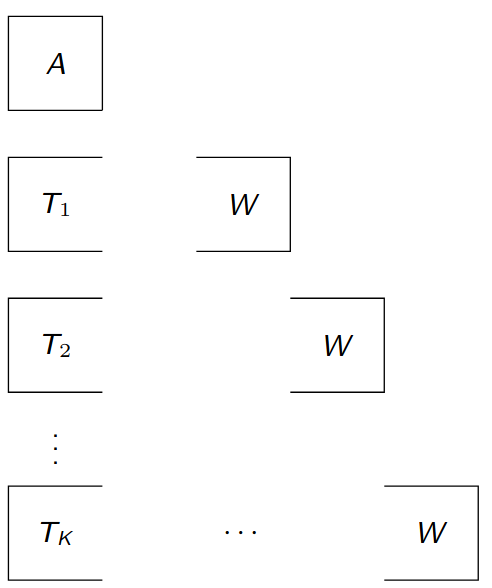
\includegraphics[width=\textwidth]{img/dw_primal.png}
		\caption{L-Shaped method (primal form)}
	\end{subfigure}
	\begin{subfigure}[b]{.5\textwidth}
		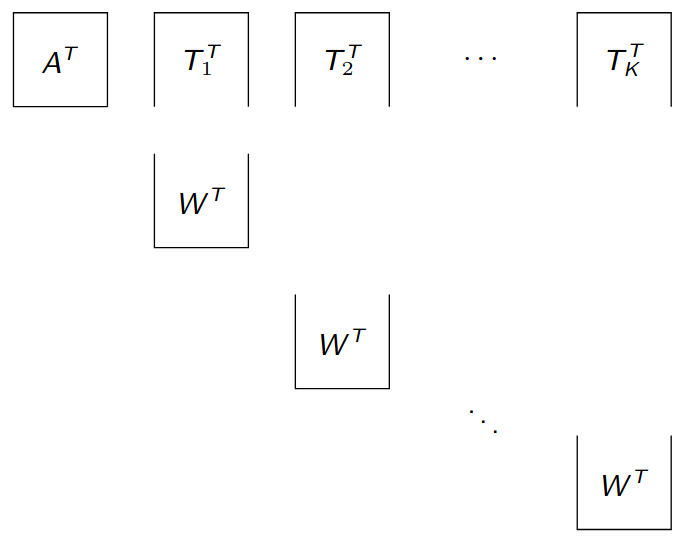
\includegraphics[width=\textwidth]{img/dw_dual.png}
		\caption{Dantzig-Wolfe method (dual form)}
	\end{subfigure}
	\caption{Comparison of the constraints}
	\label{fig:dw}
\end{figure}
\section{Problem formulation}
ith two sets of variables $x_1$ and $x_2$, our problem is 
\begin{equation}
	\begin{aligned}
		z^* &= \min_1^Tx_1 + c_2^Tx_2\\
		\text{s.t. } &Ax_1 + Bx_2 = b\\
		&B_1x_1 = d_1\\
		&B_2x_2 = d_2\\
		&x_1,x_2\ge 0
	\end{aligned}
\end{equation}
We consider $A_1x_1+A_2x_2=b$ to be the complicating constraint due to coupling. 
\subsection{Minkowski's Representation theorem}
A convex polyhedron can be characterized by equalities or by its extreme points and rays:
\begin{equation}
	\mathcal{P} = \{x\ge 0:Bx=d\} 
\end{equation}
\begin{equation}
	\mathcal{P} = \{x|\ x = \sum_{j\in J}x_j\lambda_j + \sum_{r\in R}w_r\mu_r, \ \sum_{j\in J} \lambda_j = 1, \ \mu_r,\lambda_j\ge 0\}
\end{equation}
where $x_j$ are the extreme points and $w_r$ are the extreme rays.\\
\subsection{Changing the problem with Minkowski}
Minkowski's theorem helps us rewrite the whole problem: using 
\begin{equation}
	x_1 = \sum_{j\in J_1}\lambda_1^j x_1^j + \sum_{r\in R_1}\mu_1^r w_1^r 
\end{equation}
and the same for $x_2$, we get 
\begin{equation}
	\begin{aligned}
		z &= \min \sum_{j\in J_1} \lambda_1^j c_1^Tx_1^j + \sum_{r\in R_1} \mu_1^r c_1^Tw_1^r + \sum_{j\in J_2} \lambda_2^j c_2^Tx_2^j + \sum_{r\in R_2} \mu_2^r c_2^Tw_2^r\\
		& \sum_{j\in J_1} \lambda_1^j A_1x_1^j + \sum_{r\in R_1} \mu_1^r A_1w_1^r + \sum_{j\in J_2} \lambda_2^j A_2x_2^j + \sum_{r\in R_2} \mu_2^r A_2w_2^r = b \qquad [\pi]\\
		& \sum_{j\in J_1}\lambda_1^j = 1 \qquad \qquad \qquad \qquad \qquad \qquad \qquad \qquad \qquad \qquad \qquad \quad \ [t_1]\\
		& \sum_{j\in J_2}\lambda_2^j = 1 \qquad \qquad \qquad \qquad \qquad \qquad \qquad \qquad \qquad \qquad \qquad \quad \ [t_2]\\
		& \lambda_1^j, \lambda_2^j, \mu_1^r, \mu_2^r \ge 0
	\end{aligned}
\end{equation}
This gives more variables ($|J_1|+|J_2|+|R_1|+|R_2|>n_1+n_2$), but much less constraints ($m+2>m+m_1+m_2$), where $m$ is the dimension of $b$, and $m_i$ is the dimension of $d_i$. The variables here are the weights of the extreme points and rays.\\
In matrix form, the constraints are 
\begin{equation}
	\sum_{j\in J_1} \lambda_1^j \begin{bmatrix}
		A_1 x_1^j\\ 1 \\ 0 \\
	\end{bmatrix} + \sum_{j\in J_2}\lambda_2^j \begin{bmatrix}
		A_2 x_2^j\\ 0 \\ 1 \\
	\end{bmatrix} + \sum_{r\in R_1} \mu_1^r \begin{bmatrix}
		A_1 w_1^r\\ 0 \\ 0 \\
	\end{bmatrix} + \sum_{r\in R_2} \mu_2^r \begin{bmatrix}
		A_2 w_2^r\\ 0 \\ 0 \\
	\end{bmatrix} = \begin{bmatrix}
		b\\ 1 \\ 1 \\
	\end{bmatrix}
\end{equation}
The Dantzig-Wolfe decomposition consists in solving with subsets of variables and add some little by little. 
\subsection{Reduced cost}
The certificate of optimality tells us that, given a basic feasible solution, all variables have non-negative reduced costs. Given a basis $B$\footnote{Set of variables that are non zero.}, recall that it is optimal when 
\begin{itemize}
	\item Feasibility: $x_B^* =B^{-1}b\ge 0$;
	\item Optimality: $c^T - \pi^TA \ge 0$;
\end{itemize} 
From this, the reduced cost for a basic linear program in standard form is $c^T - c^T_BB^{-1}A$.\\
From this, the reduced costs of our variables are
\begin{equation}	
	\begin{aligned}
		(c_1^T-\pi^TA_1)x_1^j - t_1 \qquad \text{ for } \lambda_1^j\\
		(c_1^T-\pi^TA_1)x_1^j \qquad \text{ for } \mu_1^j\\
	\end{aligned}
\end{equation}
and same for $x_2^j$ and $\mu_2^j$. As there is an enormous number of variables, we can solve the following problem instead of looking at all reduced costs:
\begin{equation}
	\begin{aligned}	
		z_1 &= \min(c_1^T-\pi^TA_1)x_1 \qquad \text{s.t. } B_1x_1=d_1\qquad \text{ and }x_1\ge 0\\
		z_2 &= \min(c_2^T-\pi^TA_2)x_2 \qquad \text{s.t. } B_2x_2=d_2\qquad \text{ and }x_2\ge 0\\
	\end{aligned}	
\end{equation}
For each subproblem, given their solution, we have 3 possibilities:
\begin{enumerate}
	\item The optimal cost is $-\infty$:
	\begin{itemize}
		\item Simplex output: extreme ray $w_1^r$ with $(c_1^T-\pi^TA_1)w_1^r<0$;
		\item Conclusion: the reduced cost of $\mu_1^r$ is negative;
		\item Action: We include $\mu_1^r$ in the main problem with the column
		\begin{equation}
			\begin{bmatrix}
				A_1w_1^r\\ 0 \\ 0\\
			\end{bmatrix}
		\end{equation}
	\end{itemize}
	\item The optimal cost is finite and less than $t_1$:
	\begin{itemize}
		\item Simplex output: extreme point $x_1^j$ with $(c_1^T-\pi^TA_1)x_1^j < t_1$;
		\item Conclusion: the reduced cost of $\lambda_1^j$ is negative;
		\item Action: include $\lambda_1^j$ in the main problem with the column 
		\begin{equation}
			\begin{bmatrix}
				A_1x_1^j \\ 0 \\0 \\
			\end{bmatrix}
		\end{equation}
	\end{itemize}
	\item The optimal cost is finite and bigger than $t_1$:
	\begin{itemize}
		\item Conclusion: $(c_1^T-\pi^TA_1)x_1^j\ge t_1$ for all extreme points $x_1^j$ and $(c_1^T-\pi^TA_1)w_1^r\ge 0$ for all extreme rays $w_1^r$;
		\item Action: terminate, we have an optimal basis;
	\end{itemize}
\end{enumerate}
\begin{algorithm}[H]
	\caption{Dantzig-Wolfe Decomposition Algorithm}
	\label{algo:dw}
	\begin{algorithmic}[1]
		\State \textbf{Step 1:} Solve the restricted main problem with the initial basic feasible solution, and store $(\pi,t_1,t_2)$;
		\State \textbf{Step 2:} Solve the subproblems 1 and 2;
		\If{$(c_1^T-\pi^TA_1)x\ge t_1$ and $(c_2^T-\pi^TA_2)x\ge t_2$}
		Terminate with the optimal solution:
		\begin{equation}
			\begin{aligned}
				x_1 &= \sum_{j\in \tilde J_1}\lambda_1^jx_1^j + \sum_{r\in \tilde R_1}\mu_1^r w_1^r\\
				x_2 &= \sum_{j\in \tilde J_2}\lambda_2^jx_2^j + \sum_{r\in \tilde R_2}\mu_2^r w_2^r
			\end{aligned}
		\end{equation}
		\EndIf
		\If{Subproblem $i$ is unbounded} add $\mu_i^r$ to the main problem;
		\EndIf
		\If{Subproblem $i$ has a bounded optimal cost less than $t_i$} add $\lambda_i^j$ to the main problem;\EndIf 
		\State \textbf{Step 3:} Generate the column associated with the entering variable and go back to \textbf{Step 1}.
	\end{algorithmic}
\end{algorithm}
\section{Generalisation}
The method can be generalised to $K$ subproblems:
\begin{equation}
	\begin{aligned}
		&\min c_1^T x_1 + c_2^Tx_2 + \dots + c_K^Tx_K\\
		&\text{s.t.  }A_1x_1 + A_2x_2 + \dots + A_Kx_K = b\\
		& B_i x_i = d_i \qquad i = 1,\dots,K\\
		& x_1,\dots,x_K\ge 0
	\end{aligned}
\end{equation}
\subsection{Bounds}
We denote the following:
\begin{itemize}
	\item $z_i$ the optimal objective function value of subproblem $i$;
	\item $z^*$ the optimal objective function value of the main problem;
	\item $z$ the optimal objective function value of the restricted main problem;
	\item $t_i$ the dual optimal multiplier of the constraint $\lambda_i^j$ in the restricted main problem;
\end{itemize}
At each iteration, we have the following bounds:
\begin{equation}
	z+\sum_{i=1}^K (z_i-t_i)\le z^* \le z 
\end{equation}
\section{Dantzig-Wolfe in 2-Stage Stochastic Programming}
For the Dantzig-Wolfe decomposition in stochastic programming, we use the dual problem:
\begin{equation}
	\begin{aligned}
		&\max \rho^Tb + \sum_{k=1}^K\pi_k^Th_k\\
		&\text{s.t. } \rho^T A + \sum_{k=1}^K \pi_kT_k = c^T\\
		& \pi_k^T W\le p_k q_k^T\\
	\end{aligned}
\end{equation}
where the primal is equation \ref{eq:EF}. 
Let us consider the feasible region of 
\begin{equation}
	\begin{bmatrix}
		\pi_1^T & \dots & \pi_K^T\\
	\end{bmatrix}
	\begin{bmatrix}
		W& \dots & 0\\
		0 & \dots 0\\
		0 & \dots & W\\
	\end{bmatrix}
	\le \begin{bmatrix}
		q_1^T & \dots & q_K^T\\
	\end{bmatrix}
\end{equation}
We denote $\pi^j$ as the extreme points of the region and $w_r$ as the extreme rays. We define the following quantities:
\begin{equation}
	\begin{aligned}
		E_j = (\pi^j)^T\begin{bmatrix}
			p_1 T_1\\ \vdots\\ p_K T_K\\
		\end{bmatrix} \qquad e_j = (\pi^j)^T \begin{bmatrix}
			p_1h_1\\ \vdots\\ p_Kh_K\\
		\end{bmatrix}\\
		D_r = (w^r)^T \begin{bmatrix}
			p_1 T_1\\ \vdots\\ p_K T_K\\
		\end{bmatrix}
		\qquad d_r = (w^r)^T \begin{bmatrix}
			p_1h_1\\ \vdots\\ p_Kh_K\\
		\end{bmatrix}
	\end{aligned}
\end{equation}
\subsection{Full Main Problem}
\begin{equation}\label{eq:main_dw}
	\begin{aligned}
		z^* &= \max \rho^Tb + \sum_{j\in J}\lambda^j e_j + \sum_{r\in R}\mu^r d_r\\
		& \text{s.t. }\rho^T A + \sum_{j\in J} \lambda^j E_j + \sum_{r\in R}\mu^r D_r \le c^T\\
		& \sum_{j\in J}\lambda^j = 1\\
		& \lambda^j, \mu^r \ge 0\\
	\end{aligned}
\end{equation}
Whose dual is the L-Shaped full main problem. 
\subsection{Second-Stage Subproblems}
The second-stage subproblems are
\begin{equation}\label{eq:sub_dw}
	\begin{aligned}
		z_k &= \max \pi_k^T(h_k-T_kx)\\
		& \text{s.t. } \pi_k^T W\le q_k\\
	\end{aligned}
\end{equation}
\subsection{A more specific algorithm}
\begin{algorithm}[H]
	\caption{Dantzig-Wolfe for second-stage stochastic programs}
	\label{algo:dw_sssp}
	\begin{algorithmic}[1]
		\State \textbf{Step 0:} $|\tilde J|=|\tilde R|=\nu=0$;
		\State \textbf{Step 1:} $\nu \gets \nu + 1$ and solve problem \eqref{eq:main_dw};
		\State \textbf{Step 2:} \For{$k=1,\dots,K$} solve subproblem \eqref{eq:sub_dw};
		\If{an extreme ray $w^r$ is found} set $d_{|\tilde R|+1} = (w^\nu)h_k$ and $D_{|\tilde R|+1} = (w^\nu)T_k$; 
				$|\tilde R| \gets |\tilde R| + 1$ and return to \textbf{Step 1};
		\EndIf 
		\EndFor
		\If {all subproblems are solvable} let 
		\begin{equation}
			E_{|\tilde J|+1} = \sum_{k=1}^K p_k(\pi_k^\nu)^T T_k \qquad e_{|\tilde J|+1} = \sum_{k=1}^K p_k (\pi_k^\nu)^T h_k 
		\end{equation}
		\If {$e_{|\tilde J|+1} - E_{|\tilde J|+1}x^\nu - \theta \le 0$} 
		\State Stop with $(\rho^\nu, \lambda^\nu, \mu^\nu)$ and $(x^\nu, \theta^\nu)$ optimal;
		\Else 
		\State Set $|\tilde J| \gets |\tilde J| + 1$ and go back to \textbf{Step 1}.
		\EndIf 
		\EndIf 
	\end{algorithmic}
\end{algorithm}
\subsection{And more specific bounds}
\begin{equation}
	z \le z^* \le c^Tx + \sum_{k=1}^K p_k z_k
\end{equation}
\section{Dantzig-Wolfe in Integer Programming}
\subsection{Formulation}
\begin{equation}
	\begin{aligned}
		(IP): &\ \min\{c^Tx \ : x\in X\}\\
		&X = Y\cap Z\\
		&Y = \{Dx\ge d\}\\
		&Z = \{Bx\ge b\} \cap \mathbb{Z}^n
	\end{aligned}
\end{equation}
The idea in this case is to apply Dantzig-Wolfe to $(IP)$ using Minkowski Representation Theorem to represent the convex hull of $Z$. 
\subsection{Reformulation}
If we assume that $Z$ is bounded, we can reformulate the problem as follows:
\begin{equation}\label{eq:mlp}
	\begin{aligned}
		(DWc): &\ z^{DWc} = \min_{\lambda \ge 0} \sum_{j\in J}(c^Tx^j)\lambda^j\\
		& \sum_{j\in J}(Dx^j)\lambda^j \ge d\\
		& \sum_{j\in J}\lambda^j = 1\\
		& x = \sum_{j\in J}x^j\lambda^j \in \mathbb{Z}^n
	\end{aligned}
\end{equation}
where $x^j$ is the set of extreme points of the convex hull of $Z$. The linear relaxation of $(DWc)$ is called the Main Linear Program (MLP), and its restricted version (RMLP) restricts the number of extreme points to a subset $\tilde J \subseteq J$. 
\subsection{Algorithm}
\begin{algorithm}[H]
	\caption{Column Generation Algorithm for (MLP)}
	\label{algo:col}
	\begin{algorithmic}[1]
		\State \textbf{Step 0:} Bounds $UB = +\infty$, $LB= -\infty$ and $t=0$;
		\While{$UB\neq LB$}
		\State Solve (RMLP) for $x^j$, $j\in \tilde J^t$, record the primal solution $\lambda^t$ and the dual solution $(\pi^t, \sigma^t)$;
		\State Solve the pricing problem 
		\begin{equation}
			\begin{aligned}
				(SP^t): & z^t = \min (c^T - (\pi^t)^T D)x\\
				& x\in Z
			\end{aligned}
		\end{equation}
		\State Let $x^t$ be an optimal solution.
		\If {$z^t-\sigma^t =0$} set $UB=z^{RMLP}$ and stop with optimal solution to (MLP);
		\Else \State Add $x^t$ to $\tilde J^t$ in (RMLP);
		\EndIf
		\State Compute the lower bound $LB=\max\{LB,(\pi^t)^T d+z^t\}$;
		\State $t\gets t+1$;
		\EndWhile 
	\end{algorithmic}
\end{algorithm}
\section{Relationship to Lagrangian Relaxation}
The MLP from equation \eqref{eq:mlp} can be derived using a Lagrangian relaxation. Let us relax the constraint $Dx\ge d$ while keeping the remaining constraints $Z=\{x\in \Z_+^n:Bx\ge b\}$, we get
\begin{itemize}
	\item The dual function:
	\begin{equation}
		g(\pi) = \min_x c^T x + \pi^T(Dx-d) \qquad \text{s.t. } xBx\ge b, x\in \Z_+^n
	\end{equation}
	\item The dual bound:
	\begin{equation}
		z_{LD} = \max_{\pi\ge 0} g(\pi) = \max_{\pi\ge 0} \min_{x\in Z} c^T x + \pi^T(Dx-d)
	\end{equation}
\end{itemize}
Equivalently, the dual bound can be written as
\begin{equation}
	\begin{aligned}
		z_{LD} &= \max_{\pi\ge 0}\min_{j\in J}\{c^T x^j + \pi^T(Dx^j-d)\}\\
		&= \max_{\pi\ge 0, \sigma} \pi^Td+\sigma \qquad \text{s.t. } \sigma \le c^T x_j - \pi^T Dx^j\qquad j\in J
	\end{aligned}
\end{equation}
And the dual problem of this bound is 
\begin{equation}
	\begin{aligned}
		z_{LD} &= \min_{\lambda^j\ge 0, j\in J} \sum_{j\in J}(c^Tx^j)\lambda^j\\
		&\text{s.t. } \sum_{j\in J}(Dx^j)\lambda^j \ge d\\
		& \sum_{j\in J}\lambda^j = 1\\ 
	\end{aligned}
\end{equation}
which is exactly the MLP from equation \eqref{eq:mlp}. Therefore, solving both is equivalent and gives the same bound. 
\end{document}